\documentclass[12pt,a4paper]{article}

% ── Pakiety ───────────────────────────────────────────────────────────
\usepackage[T1]{fontenc}
\usepackage[utf8]{inputenc}
\usepackage[polish]{babel}
\usepackage{geometry}
\geometry{margin=2.5cm}
\usepackage{graphicx}
\graphicspath{{../results/charts/}{./}}
\usepackage{booktabs}
\usepackage{array}
\usepackage{longtable}
\usepackage{multirow}
\usepackage{float}
\usepackage{caption}
\usepackage{subcaption}
\usepackage{hyperref}
\usepackage{listings}
\usepackage{xcolor}
\usepackage{amsmath}
\usepackage{enumitem}
\usepackage{titlesec}
\usepackage{fancyhdr}
\usepackage{indentfirst}

\setlength{\emergencystretch}{2em}
\setlength{\headheight}{14pt}

\hypersetup{
    colorlinks=true,
    linkcolor=blue!70!black,
    urlcolor=blue!60!black,
    citecolor=green!50!black,
}

\lstset{
    basicstyle=\ttfamily\footnotesize,
    breaklines=true,
    frame=single,
    backgroundcolor=\color{gray!10},
    keywordstyle=\color{blue},
    commentstyle=\color{green!50!black},
    stringstyle=\color{red!70!black},
}

\pagestyle{fancy}
\fancyhf{}
\fancyhead[L]{\small Zaawansowane Technologie Baz Danych}
\fancyhead[R]{\small Sprawozdanie projektowe}
\fancyfoot[C]{\thepage}

\title{
    \vspace{-1cm}
    \Large\textbf{Zaawansowane Technologie Baz Danych}\\[0.3cm]
    \large Porównanie wydajności systemów zarządzania bazami danych:\\
    PostgreSQL, MySQL, MongoDB, Redis\\[0.5cm]
    \normalsize Sprawozdanie projektowe
}
\author{
    Jakub Balicki\\[0.2cm]
    Politechnika Krakowska\\
    Kierunek: Informatyka
}
\date{Maj 2026}

\begin{document}

\maketitle
\thispagestyle{empty}
\newpage
\tableofcontents
\newpage

% ══════════════════════════════════════════════════════════════════════
\section{Cel i zakres pracy}
% ══════════════════════════════════════════════════════════════════════

Celem projektu jest porównanie wydajności czterech systemów zarządzania bazami danych (SZBD) przy wykonywaniu operacji CRUD: tworzenia, odczytu, aktualizacji i~usuwania danych na dużych zbiorach. Analizie poddano:

\begin{itemize}[noitemsep]
    \item \textbf{2 systemy relacyjne}: PostgreSQL 16, MySQL 8.0
    \item \textbf{2 systemy nierelacyjne}: MongoDB 7 (dokumentowa), Redis 7 (klucz-wartość)
\end{itemize}

Zakres pracy obejmuje:
\begin{enumerate}[noitemsep]
    \item Zaprojektowanie schematu danych systemu szpitalnego (13 tabel relacyjnych, model dokumentowy MongoDB, struktury klucz-wartość Redis).
    \item Implementację aplikacji testowej automatyzującej generowanie danych, wstawianie, pomiary i~analizę.
    \item Przeprowadzenie 24 scenariuszy testowych CRUD (6 na każdą operację) w~trzech skalach: 500\,000, 1\,000\,000 oraz 10\,000\,000 sumarycznych rekordów.
    \item Porównanie wydajności przed i po zastosowaniu indeksów.
    \item Analizę planów wykonania zapytań.
    \item Weryfikację hipotezy badawczej o wpływie indeksów na wydajność.
\end{enumerate}

\subsection{Hipoteza badawcza}

\textbf{H1: Indeksy a wydajność} -- Zastosowanie indeksów znacząco poprawia wydajność odczytu danych kosztem spadku wydajności wstawiania i~aktualizacji danych.


% ══════════════════════════════════════════════════════════════════════
\section{Opis wybranych systemów zarządzania bazami danych}
% ══════════════════════════════════════════════════════════════════════

\subsection{PostgreSQL 16}

PostgreSQL jest zaawansowanym, obiektowo-relacyjnym systemem baz danych o otwartym kodzie źródłowym. Oferuje pełną zgodność z ACID, zaawansowane mechanizmy indeksowania (B-tree, Hash, GIN, GiST, BRIN), obsługę JSON/JSONB, widoki zmaterializowane, partycjonowanie tabel oraz replikację logiczną i strumieniową.

\textbf{Zalety}: Zaawansowane typy danych, rozbudowany optymalizator zapytań, pełna zgodność ze standardem SQL, doskonała obsługa transakcji, MVCC (Multi-Version Concurrency Control), wsparcie dla procedur składowanych w wielu językach (PL/pgSQL, PL/Python).

\textbf{Wady}: Wyższe zużycie pamięci w porównaniu z MySQL, wolniejsze wstawianie danych masowych bez odpowiedniej konfiguracji, bardziej złożona konfiguracja.

\textbf{Zastosowania biznesowe}: Systemy finansowe, systemy ERP, analityka danych, systemy GIS (PostGIS), platformy e-commerce.

\subsection{MySQL 8.0}

MySQL jest najpopularniejszym relacyjnym systemem baz danych o otwartym kodzie. Wykorzystuje silnik InnoDB z obsługą transakcji ACID, mechanizmem MVCC, kluczami obcymi i indeksami B-tree. MySQL 8.0 wprowadził okna analityczne, CTE (Common Table Expressions) i ulepszony optymalizator.

\textbf{Zalety}: Wysoka wydajność operacji odczytu, łatwość konfiguracji, szeroka kompatybilność, duża społeczność, niskie wymagania sprzętowe.

\textbf{Wady}: Ograniczone wsparcie dla zaawansowanych typów danych, brak niektórych funkcji SQL standardu (np. pełna obsługa sekwencji), historycznie słabsza optymalizacja podzapytań.

\textbf{Zastosowania biznesowe}: Aplikacje webowe (WordPress, Joomla), systemy CMS, platformy SaaS, systemy logistyczne.

\subsection{MongoDB 7}

MongoDB jest dokumentową bazą danych NoSQL, przechowującą dane w formacie BSON (Binary JSON). Oferuje elastyczny schemat, replikację zestawów replik (Replica Sets), sharding dla skalowalności horyzontalnej oraz zaawansowane indeksowanie (pojedyncze, złożone, wielokluczowe, tekstowe, geoprzestrzenne).

\textbf{Zalety}: Elastyczny schemat (schema-less), naturalne modelowanie danych hierarchicznych, szybkie operacje na pojedynczych dokumentach, łatwa skalowalność horyzontalna, wbudowana agregacja.

\textbf{Wady}: Brak transakcji wielodokumentowych (do wersji 4.0), większe zużycie pamięci dyskowej, brak klasycznych złączeń relacyjnych (wymaga denormalizacji lub operatora \$lookup), ewentualna spójność w konfiguracjach rozproszonych.

\textbf{Zastosowania biznesowe}: Systemy zarządzania treścią, aplikacje mobilne, IoT, katalogi produktów, systemy analityki czasu rzeczywistego.

\subsection{Redis 7}

Redis (Remote Dictionary Server) jest bazą danych typu klucz-wartość działającą w pamięci RAM. Obsługuje struktury danych: stringi, hashe, listy, zbiory, zbiory uporządkowane, strumienie. Oferuje persystencję (RDB, AOF), replikację master-slave i klaster Redis.

\textbf{Zalety}: Ekstremalnie niska latencja ($<1$~ms), bogate struktury danych, atomowość operacji, Pub/Sub, obsługa TTL (Time-To-Live), skrypty Lua.

\textbf{Wady}: Ograniczona pojemność (limitowana pamięcią RAM), brak złożonych zapytań (brak SQL), brak relacji między danymi, utrata danych w razie awarii (zależy od konfiguracji persystencji).

\textbf{Zastosowania biznesowe}: Cache'owanie, sesje użytkowników, kolejki wiadomości, tablice wyników w grach, systemy czasu rzeczywistego, liczniki i metryki.


% ══════════════════════════════════════════════════════════════════════
\section{Opis zbioru danych}
% ══════════════════════════════════════════════════════════════════════

Dane testowe modelują system informatyczny szpitala. Schemat relacyjny składa się z~\textbf{13 tabel}:

\begin{table}[H]
\centering
\caption{Schemat relacyjny -- tabele systemu szpitalnego}
\label{tab:schema}
\small
\begin{tabular}{@{}llp{8cm}@{}}
\toprule
\textbf{Tabela} & \textbf{Typ} & \textbf{Opis / klucze obce} \\
\midrule
departments & Słownikowa & Oddziały szpitalne (id, name, phone) \\
specializations & Słownikowa & Specjalizacje lekarskie (id, name) \\
diseases & Słownikowa & Choroby z kodem ICD-10 (id, icd10\_code, name) \\
medical\_services & Słownikowa & Usługi medyczne z ceną bazową \\
medications & Słownikowa & Leki (id, name, active\_substance) \\
patients & Główna & Pacjenci (id, PESEL, imię, nazwisko, data ur., płeć) \\
doctors & Główna & Lekarze $\rightarrow$ departments, specializations \\
visits & Transakcyjna & Wizyty $\rightarrow$ patients, doctors \\
performed\_services & Transakcyjna & Wykonane usługi $\rightarrow$ visits, medical\_services \\
diagnoses & Transakcyjna & Diagnozy $\rightarrow$ visits, diseases \\
prescriptions & Transakcyjna & Recepty $\rightarrow$ visits \\
prescription\_items & Transakcyjna & Pozycje recept $\rightarrow$ prescriptions, medications \\
test\_results & Transakcyjna & Wyniki badań $\rightarrow$ visits \\
\bottomrule
\end{tabular}
\end{table}

\begin{figure}[H]
\centering
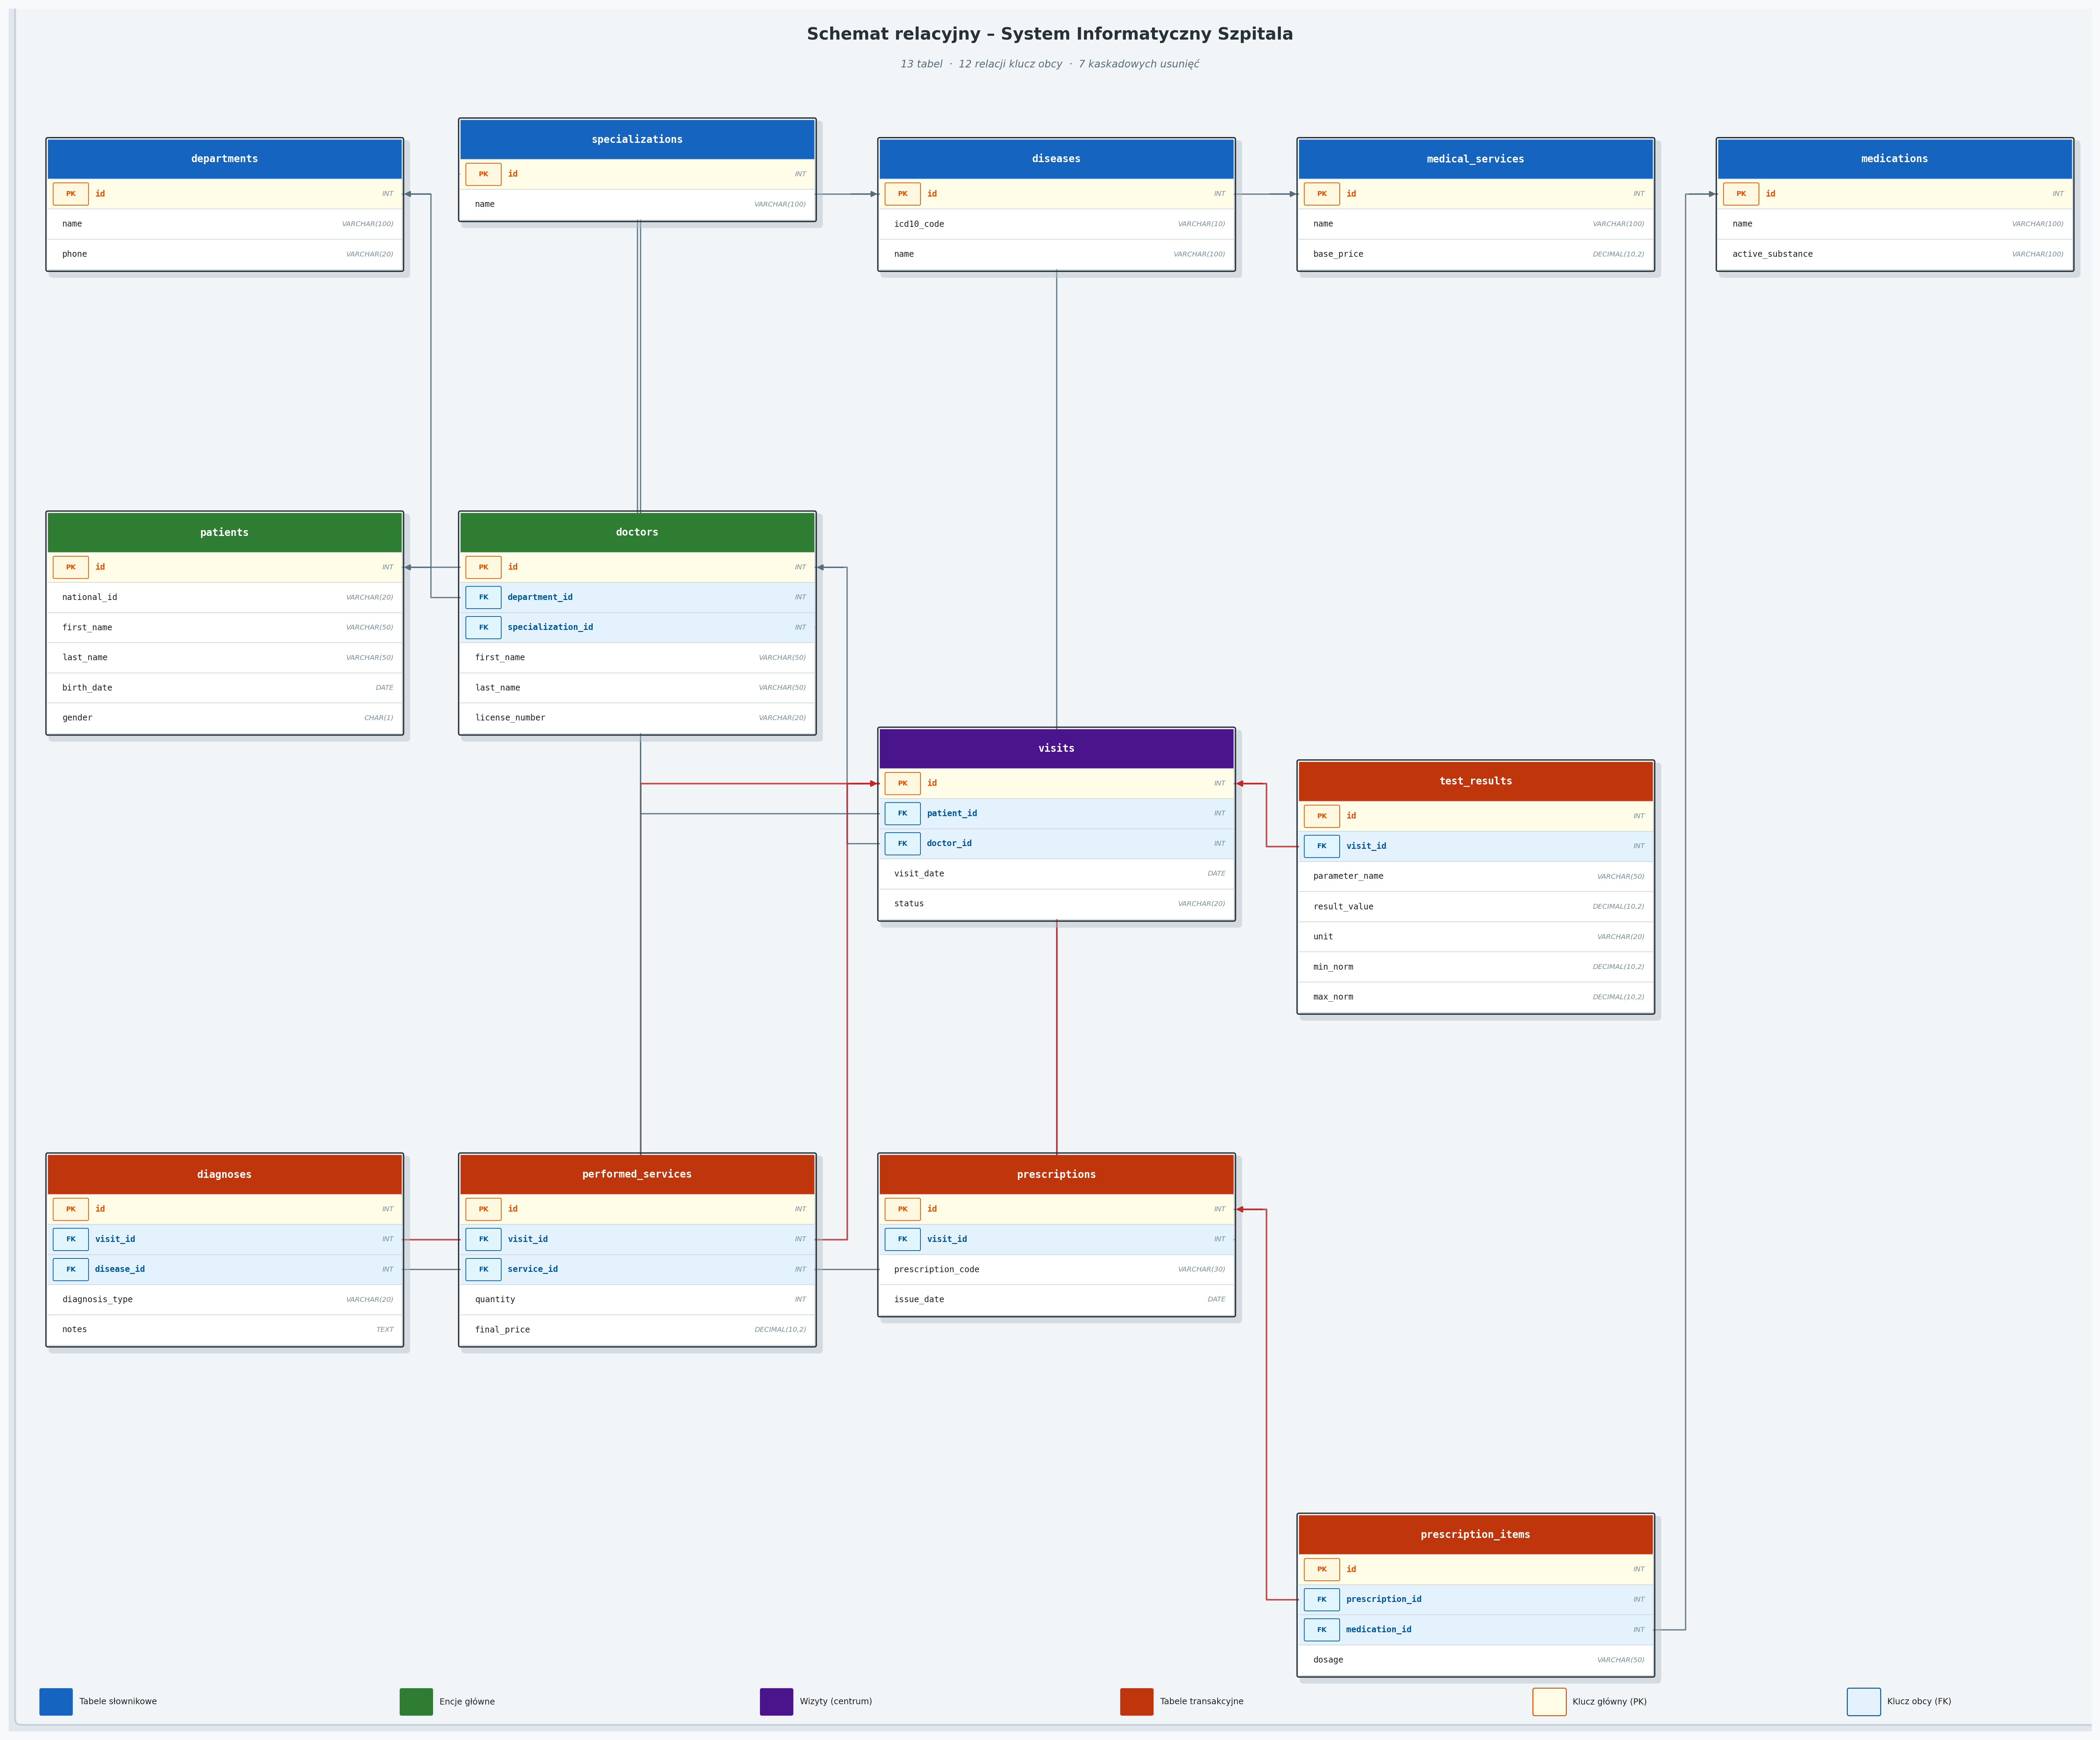
\includegraphics[width=\textwidth]{../presentation_assets/erd_diagram.png}
\caption{Diagram ERD -- schemat relacyjny systemu informatycznego szpitala}
\label{fig:erd}
\end{figure}

\subsection{Modele danych w systemach nierelacyjnych}

\textbf{MongoDB} -- model dokumentowy z zagnieżdżeniami:
Pacjent jest dokumentem głównym, zawierającym tablicę wizyt, a~każda wizyta posiada zagnieżdżone tablice: wykonane usługi, diagnozy, recepty (z~pozycjami) oraz wyniki badań. Taki model eliminuje konieczność złączeń relacyjnych, ale komplikuje aktualizację zagnieżdżonych struktur.

\textbf{Redis} -- model klucz-wartość z wieloma typami struktur:
\begin{itemize}[noitemsep]
    \item \texttt{patient:\{id\}} -- HASH z danymi pacjenta,
    \item \texttt{patient:visits:\{pid\}} -- SET identyfikatorów wizyt,
    \item \texttt{visit:status:\{id\}}, \texttt{visit:doctor:\{vid\}} -- STRING,
    \item \texttt{session:doctor:\{id\}} -- HASH z danymi lekarza,
    \item \texttt{visit:diag:\{vid\}} -- LIST diagnoz,
    \item \texttt{prescription:\{id\}}, \texttt{service:total:\{vid\}}, \texttt{department:\{id\}} -- HASH.
\end{itemize}


\subsection{Skale danych testowych}

\begin{table}[H]
\centering
\caption{Liczba rekordów w~zależności od skali}
\label{tab:scales}
\small
\begin{tabular}{@{}lrrr@{}}
\toprule
\textbf{Tabela} & \textbf{500\,000} & \textbf{1\,000\,000} & \textbf{10\,000\,000} \\
\midrule
departments & 10 & 15 & 30 \\
specializations & 15 & 20 & 40 \\
diseases & 100 & 150 & 500 \\
medical\_services & 50 & 75 & 200 \\
medications & 80 & 120 & 400 \\
patients & 8\,000 & 16\,000 & 160\,000 \\
doctors & 40 & 80 & 800 \\
visits & 100\,000 & 200\,000 & 2\,000\,000 \\
performed\_services & $\sim$100\,000 & $\sim$200\,000 & $\sim$2\,000\,000 \\
diagnoses & $\sim$100\,000 & $\sim$200\,000 & $\sim$2\,000\,000 \\
prescriptions & $\sim$40\,000 & $\sim$80\,000 & $\sim$800\,000 \\
prescription\_items & $\sim$80\,000 & $\sim$160\,000 & $\sim$1\,600\,000 \\
test\_results & $\sim$60\,000 & $\sim$120\,000 & $\sim$1\,200\,000 \\
\bottomrule
\end{tabular}
\end{table}


% ══════════════════════════════════════════════════════════════════════
\section{Opis aplikacji testowej}
% ══════════════════════════════════════════════════════════════════════

\subsection{Wymagania}
\begin{itemize}[noitemsep]
    \item Automatyczne generowanie syntetycznych danych medycznych (własny generator).
    \item Masowe wstawianie danych do 4 systemów bazodanowych.
    \item Wykonanie 24 scenariuszy CRUD w~trybie bez indeksów i~z~indeksami.
    \item Pomiar czasu operacji (średnia z~3 prób) z~dokładnością do mikrosekundy.
    \item Automatyczne generowanie raportów planów wykonania i~wykresów porównawczych.
\end{itemize}

\subsection{Wykorzystane technologie i narzędzia}
\begin{itemize}[noitemsep]
    \item \textbf{Python 3.13} -- język implementacji aplikacji.
    \item \textbf{Docker + Docker Compose} -- konteneryzacja wszystkich 4 baz danych.
    \item \textbf{psycopg2} -- sterownik PostgreSQL.
    \item \textbf{mysql-connector-python} -- sterownik MySQL.
    \item \textbf{pymongo} -- sterownik MongoDB.
    \item \textbf{redis-py} -- sterownik Redis.
    \item \textbf{pandas + matplotlib} -- analiza wyników i wizualizacja.
    \item \textbf{\LaTeX} -- skład sprawozdania.
\end{itemize}

\subsection{Struktura projektu i opis działania}
Aplikacja działa w~pełni automatycznie. Polecenie \texttt{python run\_all.py} kolejno:
\begin{enumerate}[noitemsep]
    \item Sprawdza połączenia z~bazami danych (ping).
    \item Dla każdej skali (500k, 1M, 10M): generuje dane, wstawia je do baz, uruchamia pomiary bez indeksów i~z~indeksami oraz generuje plany wykonania zapytań.
    \item Łączy wyniki CSV i~generuje wykresy porównawcze dla poszczególnych scenariuszy.
\end{enumerate}


% ══════════════════════════════════════════════════════════════════════
\section{Opis scenariuszy testowych}
% ══════════════════════════════════════════════════════════════════════

Zdefiniowano \textbf{24 scenariusze testowe} -- po 6 dla każdej operacji CRUD. Każdy scenariusz wykonywany jest 3~razy, a~raportowana jest średnia arytmetyczna czasu wykonania. Scenariusze zaprojektowano tak, aby były logicznie porównywalne między technologiami.

\begin{table}[H]
\centering
\caption{Scenariusze testowe -- operacje wstawiania danych}
\small
\begin{tabular}{@{}p{0.7cm}p{4cm}p{8.2cm}@{}}
\toprule
\textbf{Nr} & \textbf{Nazwa} & \textbf{Opis} \\
\midrule
C1 & Wstawienie pacjenta & Dodanie nowego pacjenta z~podstawowymi danymi osobowymi. \\
C2 & Wstawienie wizyty & Dodanie wizyty powiązanej z~pacjentem i~lekarzem. \\
C3 & Wstawienie diagnozy & Dodanie diagnozy przypisanej do konkretnej wizyty. \\
C4 & Wstawienie recepty z~pozycjami & Dodanie recepty oraz powiązanych pozycji leków w~jednej operacji logicznej. \\
C5 & Wstawienie wykonanej usługi & Dodanie usługi medycznej wykonanej podczas wizyty. \\
C6 & Wstawienie wyniku badania & Dodanie wyniku badania laboratoryjnego przypisanego do wizyty. \\
\bottomrule
\end{tabular}
\end{table}

\begin{table}[H]
\centering
\caption{Scenariusze testowe -- operacje odczytu danych}
\small
\begin{tabular}{@{}p{0.7cm}p{4cm}p{8.2cm}@{}}
\toprule
\textbf{Nr} & \textbf{Nazwa} & \textbf{Opis} \\
\midrule
R1 & Pobranie pacjenta po identyfikatorze & Odczyt danych jednego pacjenta wskazanego kluczem głównym lub identyfikatorem dokumentu. \\
R2 & Pobranie wizyt pacjenta z~lekarzem & Odczyt wizyt wybranego pacjenta wraz z~podstawowymi danymi lekarza. \\
R3 & Pobranie diagnoz wizyty & Odczyt diagnoz przypisanych do jednej wizyty wraz z~informacją słownikową o~chorobie. \\
R4 & Pobranie pełnej historii pacjenta & Odczyt pacjenta, wizyt, diagnoz, recept, usług i~wyników badań. \\
R5 & Wyliczenie sumy kosztów usług & Obliczenie łącznego kosztu usług medycznych wykonanych dla pacjenta. \\
R6 & Pobranie recept wraz z~lekami & Odczyt recept przypisanych do wizyty oraz powiązanych pozycji leków. \\
\bottomrule
\end{tabular}
\end{table}

\begin{table}[H]
\centering
\caption{Scenariusze testowe -- operacje aktualizacji i~usuwania danych}
\small
\begin{tabular}{@{}p{0.7cm}p{4cm}p{8.2cm}@{}}
\toprule
\textbf{Nr} & \textbf{Nazwa} & \textbf{Opis} \\
\midrule
U1 & Zmiana nazwiska pacjenta & Aktualizacja danych pacjenta wskazanego identyfikatorem. \\
U2 & Zmiana statusu wizyty & Aktualizacja statusu jednej wizyty wskazanej identyfikatorem. \\
U3 & Zmiana ceny wykonanej usługi & Aktualizacja ceny usług powiązanych z~wybraną wizytą. \\
U4 & Aktualizacja notatek diagnozy & Zmiana notatek diagnoz przypisanych do wybranej wizyty. \\
U5 & Zmiana numeru licencji lekarza & Aktualizacja numeru licencji jednego lekarza. \\
U6 & Zmiana telefonu oddziału & Aktualizacja telefonu wybranego oddziału szpitalnego. \\
\midrule
D1 & Usunięcie wyniku badania & Usunięcie pojedynczego wyniku badania bez rekordów potomnych. \\
D2 & Usunięcie diagnozy & Usunięcie pojedynczej diagnozy bez rekordów potomnych. \\
D3 & Usunięcie pacjenta & Usunięcie pacjenta wraz z~powiązanymi danymi zależnymi. \\
D4 & Usunięcie wykonanej usługi & Usunięcie pojedynczej usługi wykonanej podczas wizyty. \\
D5 & Usunięcie recepty & Usunięcie recepty wraz z~jej pozycjami. \\
D6 & Kaskadowe usunięcie wizyty & Usunięcie wizyty oraz wszystkich powiązanych z~nią danych klinicznych. \\
\bottomrule
\end{tabular}
\end{table}


% ══════════════════════════════════════════════════════════════════════
\section{Metodyka pomiaru}
\label{sec:method}
% ══════════════════════════════════════════════════════════════════════

\subsection{Schemat pomiaru}

Każdy z~24 scenariuszy CRUD (po 6 dla tworzenia, odczytu, aktualizacji i~usuwania danych) wykonano dla każdej bazy w~dwóch wariantach -- \emph{bez~indeksów} i~\emph{z~indeksami} -- oraz dla trzech skal danych: \textbf{500\,000}, \textbf{1\,000\,000} oraz \textbf{10\,000\,000} sumarycznych rekordów. Przed pomiarem wykonywany jest jeden przebieg rozgrzewający, a~następnie 3~powtórzenia, z~których wyliczana jest średnia arytmetyczna oraz odchylenie standardowe (kolumny \texttt{Average\_Time\_Seconds} i~\texttt{StdDev\_Time\_Seconds} w~\texttt{results/results\_all.csv}; w~kolumnie \texttt{Median\_Time\_Seconds} dostępna jest mediana kontrolna). Wszystkie wartości w~niniejszym rozdziale podawane są w~milisekundach [ms].

Dla scenariuszy wstawiania i~usuwania mierzony jest wyłącznie czas operacji docelowej -- odpowiednio wstawienie nowego rekordu oraz usunięcie istniejącego rekordu. Operacja komplementarna potrzebna do utrzymania stałej liczby wierszy między próbami jest wykonywana w~osobnej fazie i~nie wpływa na raportowany czas.

\subsection{Środowisko testowe}
\label{sec:env}

Pomiary wykonano na pojedynczej maszynie z~Windows~11 + WSL2 i~Docker~Desktop. Klient pomiarowy (Python~3.13) działał natywnie na hoście Windows i~łączył się z~bazami przez \texttt{localhost}. Konfiguracja kontenerów (\texttt{docker-compose.yml}) została celowo \emph{zrównana} między PostgreSQL, MySQL i~MongoDB: każdy silnik dyskowy ma 4~GB pamięci podręcznej oraz aktywną pełną synchronizację dyskową przy zatwierdzaniu transakcji. Pozwala to porównywać silniki na zbliżonym budżecie pamięci i~przy identycznej polityce trwałości transakcji:

\begin{table}[H]
\centering
\caption{Parametry uruchomieniowe kontenerów (\texttt{docker-compose.yml})}
\label{tab:env}
\small
\begin{tabular}{@{}llp{8cm}@{}}
\toprule
\textbf{Baza} & \textbf{Wersja} & \textbf{Parametry uruchomieniowe} \\
\midrule
PostgreSQL & 16 & 4~GB bufora współdzielonego, 64~MB pamięci roboczej, synchroniczne zatwierdzanie transakcji, maksymalnie 2 procesy równoległe na zapytanie \\
MySQL & 8.0 & 4~GB puli buforów InnoDB, dziennik 512~MB, synchronizacja dziennika przy każdym zatwierdzeniu transakcji, pakiety do 256~MB \\
MongoDB & 7 & 4~GB pamięci podręcznej WiredTiger, dziennik operacji aktywny domyślnie \\
Redis & 7 & limit pamięci 10~GB, brak wyrzucania kluczy, persystencja wyłączona \\
\bottomrule
\end{tabular}
\end{table}

Po wypełnieniu baz danymi oraz po dodaniu indeksów program pomiarowy wywołuje jawne \texttt{ANALYZE} (PostgreSQL) i~\texttt{ANALYZE TABLE} (MySQL), zapewniając aktualność statystyk optymalizatora. W~trakcie pojedynczego przebiegu aktywna jest tylko jedna baza naraz.

\subsection{Ograniczenia i zastrzeżenia interpretacyjne}

\begin{itemize}[noitemsep]
    \item \textbf{Liczba prób n=3}: średnia z~3 powtórzeń jest wrażliwa na pojedyncze odstające pomiary (GC pause, cache miss). Różnice $<$5\% między bazami należy traktować jako szum pomiarowy; brak możliwości rygorystycznych testów statystycznych typu t-Student/ANOVA (wymagałyby n$\geq$30).
    \item \textbf{Redis vs bazy dyskowe}: Redis pracuje wyłącznie w~RAM, z~wyłączoną persystencją -- nie wykonuje I/O dyskowych ani nie prowadzi dziennika transakcji. Bezpośrednie porównanie bezwzględnych czasów Redis z~PG/MySQL/Mongo ilustruje raczej \emph{różnicę paradygmatów} (RAM vs dysk) niż jakość implementacji.
    \item \textbf{Indeksy w~Redis}: Redis nie posiada mechanizmu indeksów -- dostęp jest deterministyczny O(1) lub O(N) wynikający z~typu struktury danych. Z~tego powodu Redis jest \textbf{wyłączony z~wykresów} porównawczych typu „bez/z~indeksami''; w~tabelach z~indeksami pojawia się jako \texttt{---}.
    \item \textbf{Asymetria odczytu dla Redis}: pobranie wizyt pacjenta z~danymi lekarza oraz wyliczenie sumy kosztów usług w~Redis ograniczają próbkę kluczy do stałej liczby elementów. Bazy SQL i~MongoDB wykonują pełne złączenia lub agregacje z~limitem 50 rekordów, dlatego przy rosnącej skali ich koszt rośnie, a~koszt Redis pozostaje stały.
    \item \textbf{Ograniczenie modelu MongoDB}: generator nakłada limit 200 wizyt na pacjenta, aby pojedynczy dokument z~zagnieżdżonymi wizytami nie przekroczył limitu BSON 16~MB. Przy testowanych skalach średnia wynosi 12--13 wizyt/pacjenta (np.\ 2~mln wizyt na 160~tys.\ pacjentów przy 10M), więc limit praktycznie nigdy nie jest aktywny i~nie wpływa na rozkład danych. MongoDB testowane jest na identycznym wolumenie rekordów co PostgreSQL i~MySQL.
\end{itemize}


% ══════════════════════════════════════════════════════════════════════
\section{Wyniki testów wydajnościowych}
\label{sec:results}
% ══════════════════════════════════════════════════════════════════════

Każda wartość w~tabelach to średnia arytmetyczna z~3~prób w~milisekundach [ms]; wartość pogrubiona w~wierszu oznacza najszybszą bazę dla danej skali i~scenariusza. Pełne wyniki (wszystkie skale + odchylenie standardowe + mediana kontrolna) znajdują się w~\texttt{results/results\_all.csv}.

\subsection{Operacja wstawiania danych}
\label{sec:res_create}

Mierzymy czas pojedynczego wstawienia wiersza; w~scenariuszu wstawienia recepty z~pozycjami obejmuje to dodanie recepty oraz jej pozycji w~jednej transakcji. Każda wartość jest średnią z~3~powtórzeń wyrażoną w~milisekundach.

\textbf{Czas wykonania bez indeksów}

\begin{table}[H]
\centering
\caption{Czas operacji wstawiania danych [ms] -- bez indeksow. Najlepszy wynik w~wierszu pogrubiony.}
\label{tab:create_no}
\small
\begin{tabular}{@{}llrrrr@{}}
\toprule
\textbf{Scenariusz} & \textbf{Skala} & \textbf{PostgreSQL} & \textbf{MySQL} & \textbf{MongoDB} & \textbf{Redis} \\
\midrule
\multirow{3}{*}{\shortstack[l]{Wstawienie\\diagnozy}}
 & 500k & 1.10 & 5.28 & 0.72 & \textbf{0.40} \\
 & 1M & 1.04 & 5.07 & 0.74 & \textbf{0.39} \\
 & 10M & 1.05 & 4.25 & 0.74 & \textbf{0.40} \\
\midrule
\multirow{3}{*}{\shortstack[l]{Wstawienie\\pacjenta}}
 & 500k & 1.03 & 4.24 & 0.70 & \textbf{0.46} \\
 & 1M & 1.12 & 4.21 & 0.69 & \textbf{0.45} \\
 & 10M & 1.19 & 3.99 & 0.84 & \textbf{0.45} \\
\midrule
\multirow{3}{*}{\shortstack[l]{Wstawienie\\wykonanej usługi}}
 & 500k & 1.06 & 5.82 & 0.74 & \textbf{0.46} \\
 & 1M & 1.02 & 4.59 & 0.79 & \textbf{0.53} \\
 & 10M & 1.06 & 6.81 & 0.85 & \textbf{0.47} \\
\midrule
\multirow{3}{*}{\shortstack[l]{Wstawienie recepty\\z pozycjami}}
 & 500k & 2.16 & 8.31 & 0.72 & \textbf{0.44} \\
 & 1M & 2.44 & 8.70 & 0.72 & \textbf{0.43} \\
 & 10M & 2.28 & 10.97 & 0.75 & \textbf{0.47} \\
\midrule
\multirow{3}{*}{\shortstack[l]{Wstawienie\\wyniku badania}}
 & 500k & 1.26 & 4.98 & 0.74 & \textbf{0.49} \\
 & 1M & 1.03 & 4.46 & 0.71 & \textbf{0.43} \\
 & 10M & 1.30 & 7.48 & 0.72 & \textbf{0.41} \\
\midrule
\multirow{3}{*}{\shortstack[l]{Wstawienie\\wizyty}}
 & 500k & 1.16 & 4.37 & 0.77 & \textbf{0.54} \\
 & 1M & 1.13 & 3.80 & 0.75 & \textbf{0.44} \\
 & 10M & 1.25 & 4.45 & 0.93 & \textbf{0.48} \\
\bottomrule
\end{tabular}
\end{table}


\textbf{Czas wykonania z~indeksami}

\begin{table}[H]
\centering
\caption{Czas operacji wstawiania danych [ms] -- z~indeksami. Najlepszy wynik w~wierszu pogrubiony. Redis nie posiada mechanizmu indeksow (kolumna `---').}
\label{tab:create_idx}
\small
\begin{tabular}{@{}llrrrr@{}}
\toprule
\textbf{Scenariusz} & \textbf{Skala} & \textbf{PostgreSQL} & \textbf{MySQL} & \textbf{MongoDB} & \textbf{Redis} \\
\midrule
\multirow{3}{*}{\shortstack[l]{Wstawienie\\diagnozy}}
 & 500k & 1.14 & 4.98 & \textbf{0.87} & --- \\
 & 1M & 1.12 & 4.38 & \textbf{0.81} & --- \\
 & 10M & 1.11 & 4.99 & \textbf{0.83} & --- \\
\midrule
\multirow{3}{*}{\shortstack[l]{Wstawienie\\pacjenta}}
 & 500k & 1.09 & 4.57 & \textbf{0.76} & --- \\
 & 1M & 1.04 & 4.34 & \textbf{0.68} & --- \\
 & 10M & 1.06 & 4.23 & \textbf{0.70} & --- \\
\midrule
\multirow{3}{*}{\shortstack[l]{Wstawienie\\wykonanej usługi}}
 & 500k & 1.16 & 4.89 & \textbf{0.70} & --- \\
 & 1M & 1.08 & 4.53 & \textbf{0.72} & --- \\
 & 10M & 1.10 & 4.15 & \textbf{0.82} & --- \\
\midrule
\multirow{3}{*}{\shortstack[l]{Wstawienie recepty\\z pozycjami}}
 & 500k & 2.09 & 8.89 & \textbf{0.70} & --- \\
 & 1M & 2.05 & 8.57 & \textbf{0.81} & --- \\
 & 10M & 2.10 & 7.70 & \textbf{0.73} & --- \\
\midrule
\multirow{3}{*}{\shortstack[l]{Wstawienie\\wyniku badania}}
 & 500k & 1.06 & 5.01 & \textbf{0.77} & --- \\
 & 1M & 1.04 & 5.46 & \textbf{0.72} & --- \\
 & 10M & 1.15 & 4.15 & \textbf{0.73} & --- \\
\midrule
\multirow{3}{*}{\shortstack[l]{Wstawienie\\wizyty}}
 & 500k & 1.17 & 5.47 & \textbf{0.85} & --- \\
 & 1M & 1.07 & 4.79 & \textbf{0.92} & --- \\
 & 10M & 1.10 & 4.40 & \textbf{0.87} & --- \\
\bottomrule
\end{tabular}
\end{table}


\subsubsection*{Porównanie baz na trzech skalach}

\begin{figure}[H]
\centering
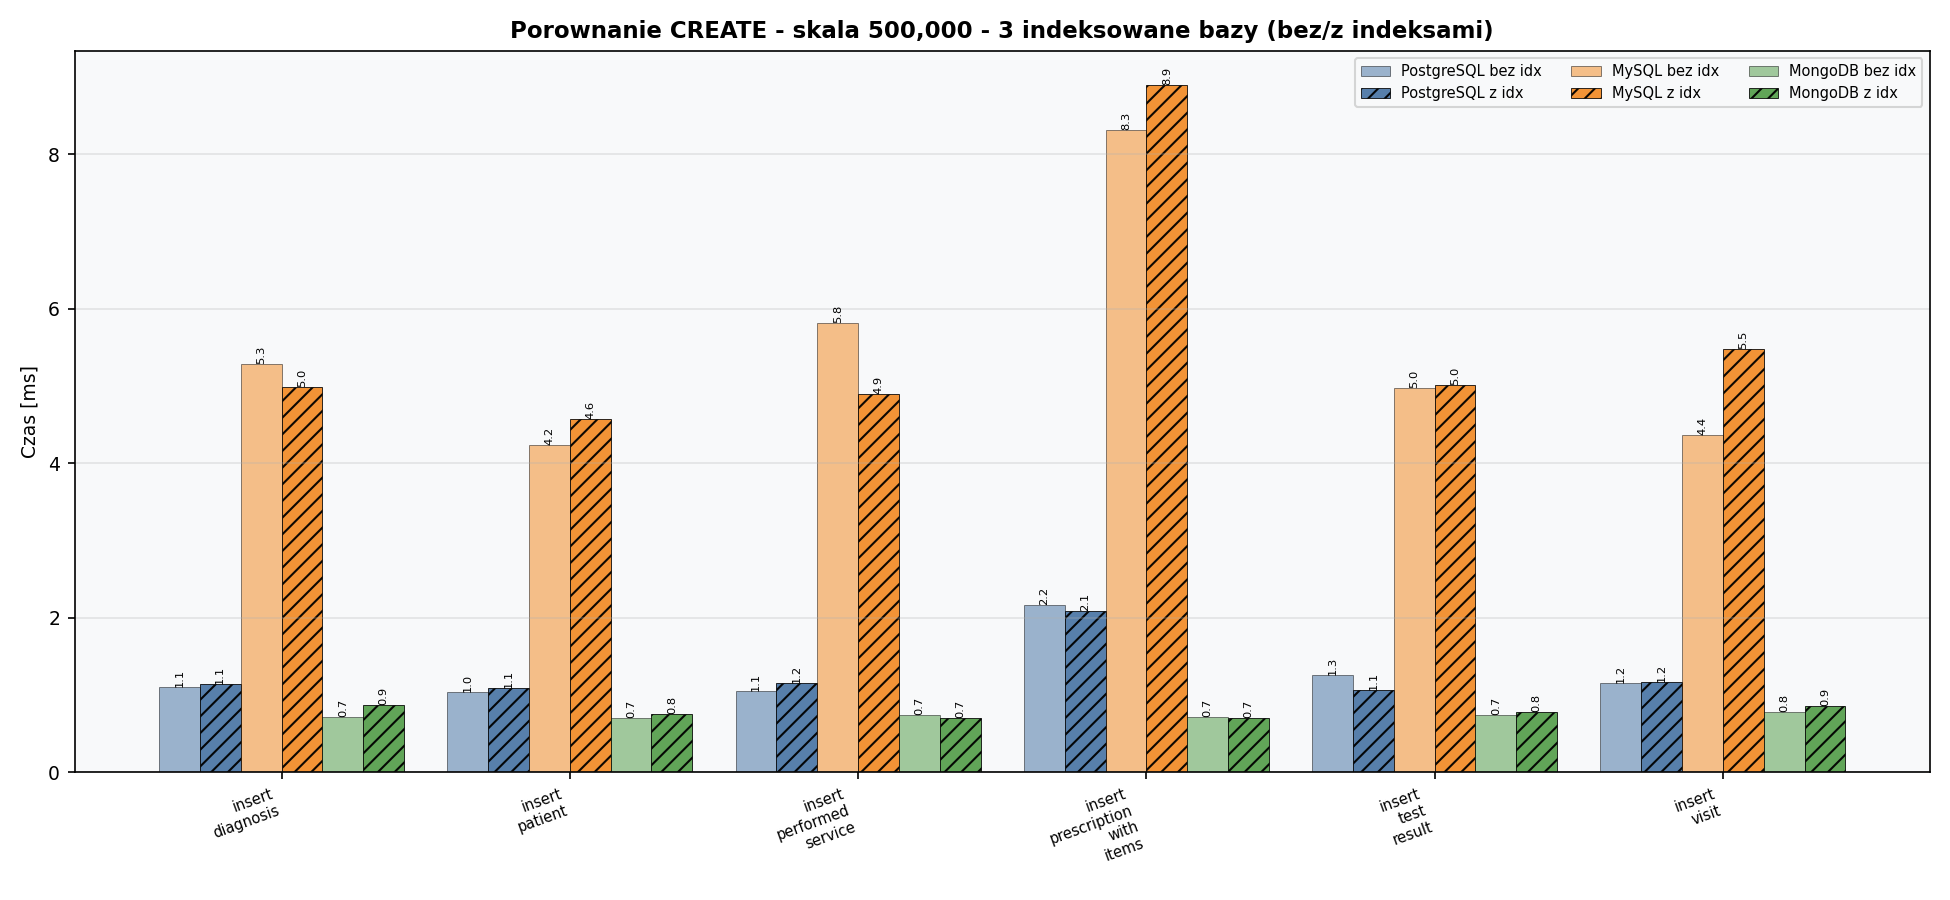
\includegraphics[width=0.95\textwidth]{crud_pair_CREATE_500000.png}
\caption{Wstawianie danych -- skala 500\,000. Każda baza ma parę wyników: wariant bez indeksów oraz wariant z~indeksami.}
\label{fig:cp_create_500k}
\end{figure}

\paragraph{Interpretacja wyników.}
Na skali 500\,000 rekordów czasy wstawiania są krótkie i~mało zależne od obecności indeksów. MongoDB pozostaje na poziomie około 0.7--0.9~ms, PostgreSQL najczęściej 1--2~ms, a~MySQL 4--9~ms. Najwolniejsze jest wstawienie recepty z~pozycjami, ponieważ obejmuje kilka powiązanych rekordów w~jednej operacji logicznej. Dane nie pokazują jednak prostego schematu ,,indeksy spowalniają wstawianie'': różnice między wariantami są niewielkie, czasem korzystne, czasem niekorzystne, a~dla MongoDB i~PostgreSQL mieszczą się blisko szumu pomiarowego.

\begin{figure}[H]
\centering
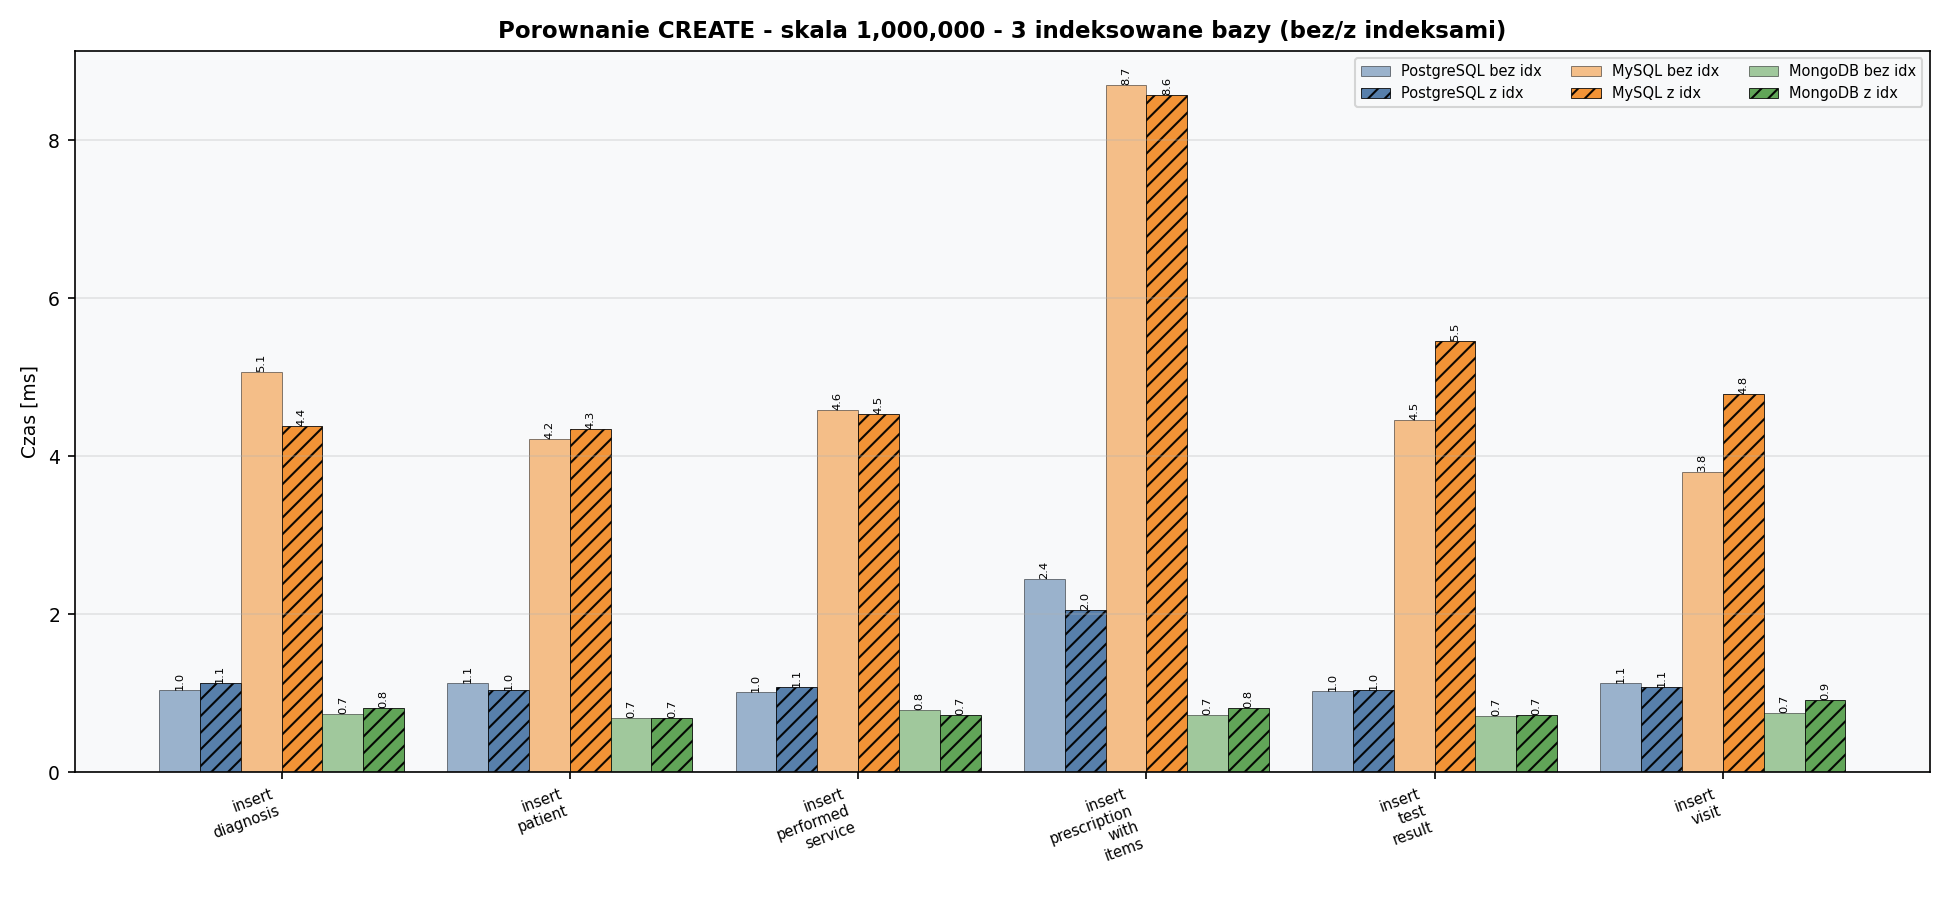
\includegraphics[width=0.95\textwidth]{crud_pair_CREATE_1000000.png}
\caption{Wstawianie danych -- skala 1\,000\,000.}
\label{fig:cp_create_1m}
\end{figure}

\paragraph{Interpretacja wyników.}
Przy 1\,000\,000 rekordów układ wyników jest analogiczny do skali 500\,000: wzrost wolumenu danych nie powoduje systematycznego wzrostu czasu pojedynczego wstawienia. Ważniejsze od skali okazują się cechy silnika i~koszt trwałego zapisu. MySQL pozostaje wyraźnie wolniejszy od pozostałych systemów, natomiast MongoDB utrzymuje najniższe czasy. Wariant z~indeksami nie tworzy jednolitego trendu: dla jednych scenariuszy jest minimalnie szybszy, dla innych minimalnie wolniejszy.

\begin{figure}[H]
\centering
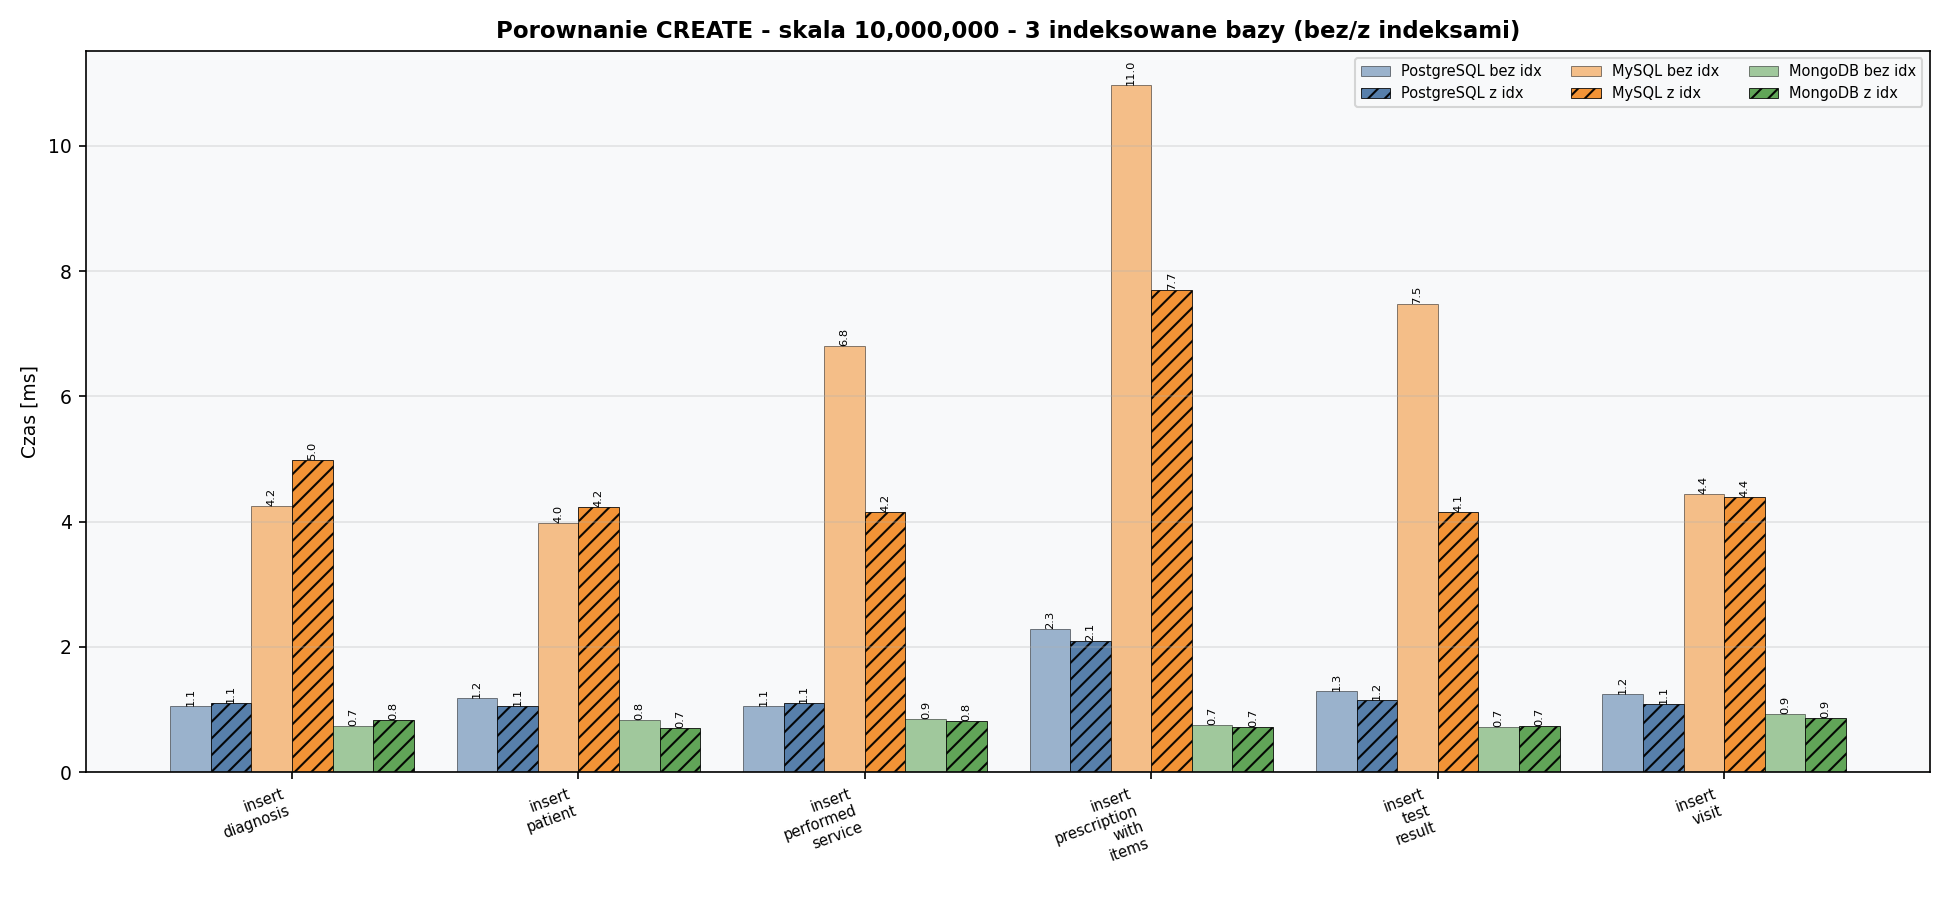
\includegraphics[width=0.95\textwidth]{crud_pair_CREATE_10000000.png}
\caption{Wstawianie danych -- skala 10\,000\,000.}
\label{fig:cp_create_10m}
\end{figure}

\paragraph{Interpretacja wyników.}
Na skali 10\,000\,000 rekordów nadal nie widać liniowego wzrostu czasu wstawiania. Najważniejszym wyjątkiem jest MySQL przy wstawieniu recepty z~pozycjami: wariant z~indeksami skraca czas z~10.97~ms do 7.70~ms. Nie jest to dowód, że indeksy ogólnie przyspieszają zapis, lecz efekt konkretnego scenariusza, w~którym sprawdzanie powiązań między receptą i~pozycjami recepty ma zauważalny koszt. Dla pozostałych przypadków wyniki są mieszane i~nie uzasadniają tezy o~stałym spowolnieniu ani stałym przyspieszeniu wstawiania.

\subsubsection*{Analiza planów wykonania -- wstawianie danych}

Plany wykonania wstawiania są proste we wszystkich silnikach SQL: pojedyncza operacja zapisu do tabeli poprzedzona ewentualnym sprawdzeniem kluczy obcych. Na poziomie planu wykonania nie ma więc złożonego wyboru ścieżki dostępu -- przy wstawianiu danych liczy się przede wszystkim koszt fizycznego zapisu, a~nie sposób wyszukiwania rekordów. Realny koszt każdego wstawienia to suma:

\begin{itemize}[noitemsep]
    \item zapisu wiersza do struktury tabeli (drzewo klastrowane w~InnoDB, sterta w~PostgreSQL, dokument BSON w~MongoDB, struktura haszująca w~Redis),
    \item dopisania nowego klucza do każdego istniejącego indeksu wtórnego,
    \item zapisu do dziennika transakcji (WAL w~PostgreSQL, dziennik odtwarzania w~MySQL, dziennik operacji w~MongoDB),
    \item synchronizacji dyskowej przy zatwierdzeniu transakcji -- w~PostgreSQL zbiorowej dla wielu transakcji, w~MySQL pojedynczej dla każdej, zgodnie z~konfiguracją z~Tabeli~\ref{tab:env},
    \item walidacji kluczy obcych po stronie tabeli docelowej (wymaga indeksu na referowanej kolumnie -- w~MySQL zawsze istnieje, w~PG tylko jeśli go utworzymy).
\end{itemize}

Większość obserwowanej różnicy między bazami pochodzi z~dwóch ostatnich pozycji: MySQL płaci za pełną synchronizację przy każdym zatwierdzeniu transakcji, dlatego jest najwolniejszy, a~MongoDB i~Redis mają lżejszą politykę trwałości. Szczegółową analizę narzutu indeksów na zapis przedstawia współczynnik $K_{zapis}$ w~Sekcji~\ref{sec:kwrite}.

\subsubsection*{Wnioski -- operacje wstawiania danych}

\begin{itemize}[noitemsep]
    \item \textbf{Wstawianie danych nie potwierdza jednoznacznie części hipotezy o~spowolnieniu zapisu}. W~badanych danych wpływ indeksów jest mały albo mieszany; nie pojawia się regularny wzrost czasu wraz ze skalą.
    \item \textbf{Różnice między silnikami są większe niż różnice między wariantami indeksowania}: MongoDB ma najniższe czasy, PostgreSQL pozostaje stabilny w~zakresie około 1--2~ms, a~MySQL jest najwolniejszy przez koszt trwałego zatwierdzania transakcji.
    \item \textbf{Wstawienie recepty z~pozycjami jest najcięższym scenariuszem w~bazach relacyjnych}. Wynika to z~kilku zapisów i~sprawdzenia powiązań, a~nie z~samego rozmiaru bazy.
    \item \textbf{Wniosek praktyczny}: dla obciążeń zdominowanych przez dopisywanie danych ważniejsza jest konfiguracja trwałości, liczba rekordów zapisywanych w~jednej operacji i~sposób obsługi powiązań niż sama obecność indeksów dodatkowych.
\end{itemize}

\subsection{Operacja odczytu danych}
\label{sec:res_read}

Mierzymy czas pojedynczego odczytu danych: od prostego pobrania rekordu po identyfikatorze po złączenia kilku tabel z~agregacją. Każda wartość to średnia z~3~powtórzeń [ms].

\textbf{Czas wykonania bez indeksów}

\begin{table}[H]
\centering
\caption{Czas operacji odczytu danych [ms] -- bez indeksow. Najlepszy wynik w~wierszu pogrubiony.}
\label{tab:read_no}
\small
\begin{tabular}{@{}llrrrr@{}}
\toprule
\textbf{Scenariusz} & \textbf{Skala} & \textbf{PostgreSQL} & \textbf{MySQL} & \textbf{MongoDB} & \textbf{Redis} \\
\midrule
\multirow{3}{*}{\shortstack[l]{Suma kosztów\\usług pacjenta}}
 & 500k & 8.50 & 1.41 & 0.75 & \textbf{0.69} \\
 & 1M & 13.55 & 1.39 & 0.77 & \textbf{0.62} \\
 & 10M & 84.85 & 1.50 & 0.76 & \textbf{0.56} \\
\midrule
\multirow{3}{*}{\shortstack[l]{Pobranie pacjenta\\po identyfikatorze}}
 & 500k & \textbf{0.41} & 1.23 & 0.77 & 0.46 \\
 & 1M & 0.41 & 1.25 & 0.77 & \textbf{0.41} \\
 & 10M & 0.48 & 1.35 & 0.89 & \textbf{0.42} \\
\midrule
\multirow{3}{*}{\shortstack[l]{Pełna historia\\pacjenta}}
 & 500k & 8.58 & 1.46 & \textbf{0.77} & 1.06 \\
 & 1M & 13.85 & 1.42 & \textbf{0.73} & 0.83 \\
 & 10M & 84.63 & 1.94 & \textbf{0.79} & 0.83 \\
\midrule
\multirow{3}{*}{\shortstack[l]{Recepty\\z lekami}}
 & 500k & 4.27 & 1.29 & 0.83 & \textbf{0.16} \\
 & 1M & 5.55 & 1.29 & 0.75 & \textbf{0.00} \\
 & 10M & 49.29 & 1.23 & 0.86 & \textbf{0.44} \\
\midrule
\multirow{3}{*}{\shortstack[l]{Diagnozy\\wizyty}}
 & 500k & 3.65 & 1.22 & 0.85 & \textbf{0.17} \\
 & 1M & 6.88 & 1.17 & 0.85 & \textbf{0.28} \\
 & 10M & 46.25 & 1.20 & 0.96 & \textbf{0.28} \\
\midrule
\multirow{3}{*}{\shortstack[l]{Wizyty pacjenta\\z lekarzem}}
 & 500k & 3.80 & 1.49 & 1.71 & \textbf{1.35} \\
 & 1M & 8.97 & 1.40 & 2.02 & \textbf{1.26} \\
 & 10M & 45.48 & 1.47 & 9.21 & \textbf{1.28} \\
\bottomrule
\end{tabular}
\end{table}


\textbf{Czas wykonania z~indeksami}

\begin{table}[H]
\centering
\caption{Czas operacji odczytu danych [ms] -- z~indeksami. Najlepszy wynik w~wierszu pogrubiony. Redis nie posiada mechanizmu indeksow (kolumna `---').}
\label{tab:read_idx}
\small
\begin{tabular}{@{}llrrrr@{}}
\toprule
\textbf{Scenariusz} & \textbf{Skala} & \textbf{PostgreSQL} & \textbf{MySQL} & \textbf{MongoDB} & \textbf{Redis} \\
\midrule
\multirow{3}{*}{\shortstack[l]{Suma kosztów\\usług pacjenta}}
 & 500k & 0.79 & 1.44 & \textbf{0.78} & --- \\
 & 1M & \textbf{0.71} & 1.36 & 0.92 & --- \\
 & 10M & 1.32 & 1.41 & \textbf{0.80} & --- \\
\midrule
\multirow{3}{*}{\shortstack[l]{Pobranie pacjenta\\po identyfikatorze}}
 & 500k & \textbf{0.49} & 1.33 & 0.79 & --- \\
 & 1M & \textbf{0.41} & 1.28 & 0.80 & --- \\
 & 10M & \textbf{0.43} & 1.24 & 0.89 & --- \\
\midrule
\multirow{3}{*}{\shortstack[l]{Pełna historia\\pacjenta}}
 & 500k & 0.83 & 1.59 & \textbf{0.76} & --- \\
 & 1M & 1.01 & 1.62 & \textbf{0.97} & --- \\
 & 10M & 1.45 & 1.67 & \textbf{0.77} & --- \\
\midrule
\multirow{3}{*}{\shortstack[l]{Recepty\\z lekami}}
 & 500k & \textbf{0.64} & 1.23 & 0.75 & --- \\
 & 1M & \textbf{0.56} & 1.31 & 0.98 & --- \\
 & 10M & \textbf{0.68} & 1.54 & 0.80 & --- \\
\midrule
\multirow{3}{*}{\shortstack[l]{Diagnozy\\wizyty}}
 & 500k & \textbf{0.55} & 1.28 & 0.85 & --- \\
 & 1M & \textbf{0.48} & 1.28 & 1.57 & --- \\
 & 10M & \textbf{0.76} & 1.26 & 0.89 & --- \\
\midrule
\multirow{3}{*}{\shortstack[l]{Wizyty pacjenta\\z lekarzem}}
 & 500k & \textbf{0.56} & 1.62 & 1.43 & --- \\
 & 1M & \textbf{0.59} & 1.51 & 1.50 & --- \\
 & 10M & \textbf{0.69} & 1.50 & 1.55 & --- \\
\bottomrule
\end{tabular}
\end{table}


\subsubsection*{Porównanie baz na trzech skalach}

\begin{figure}[H]
\centering
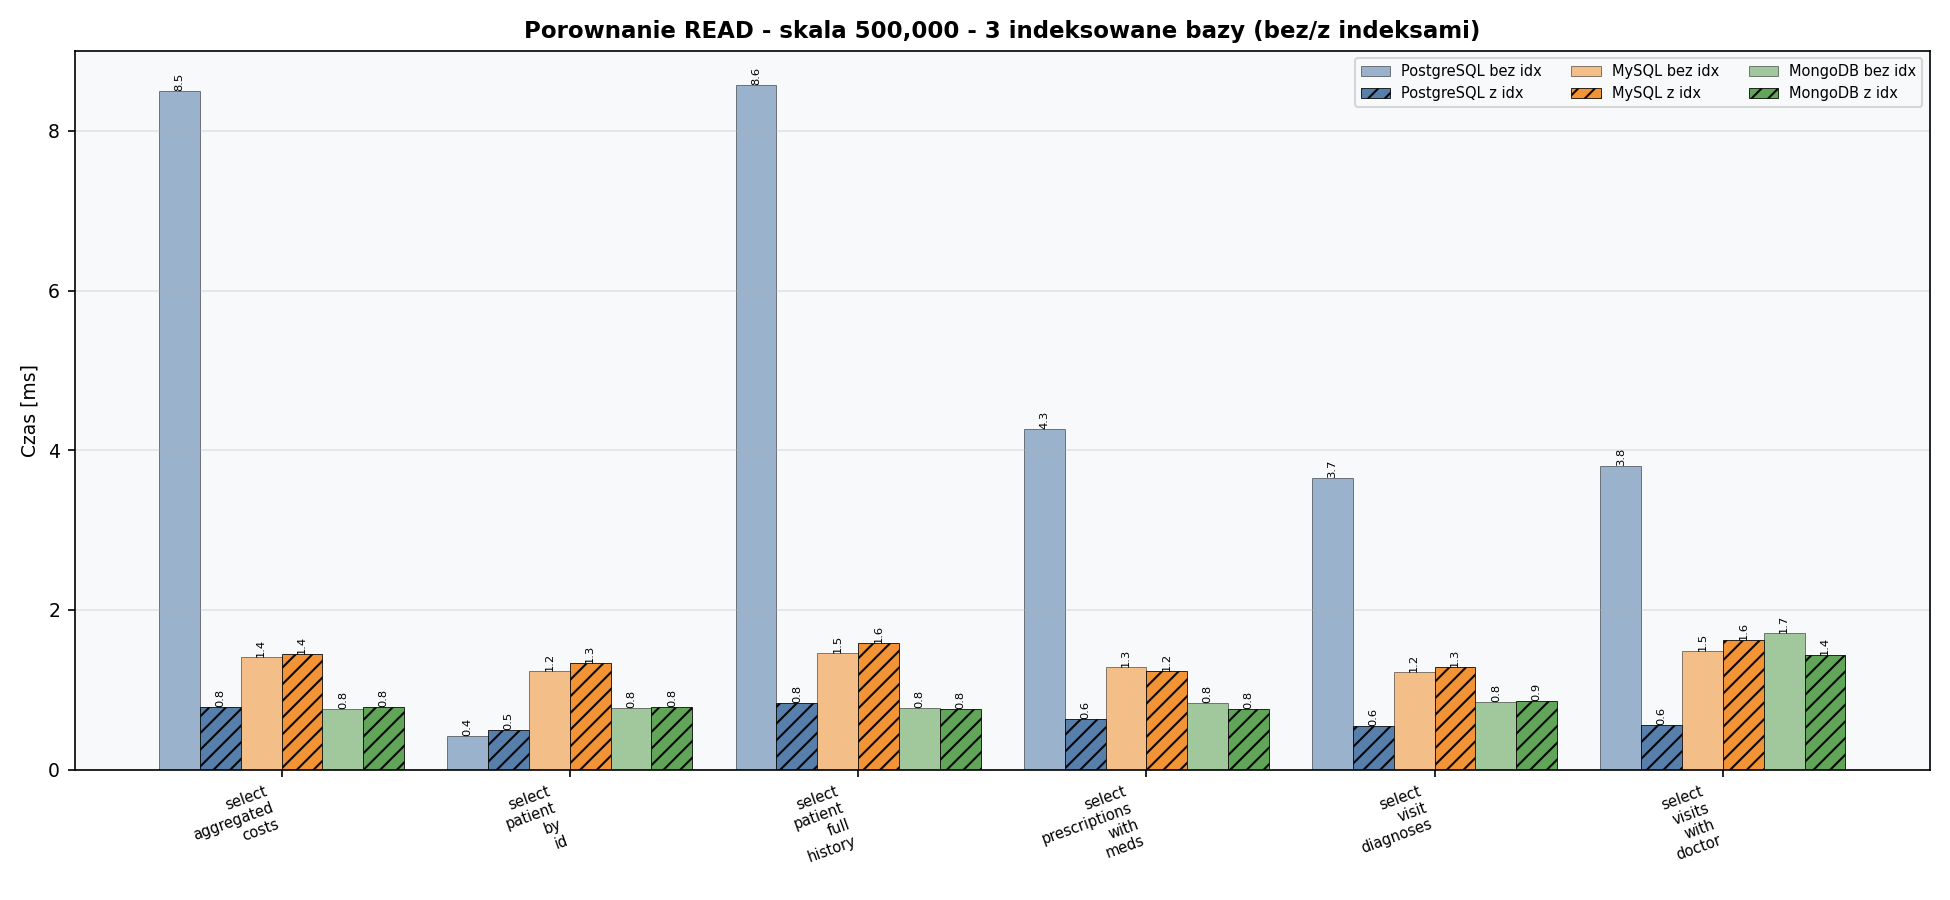
\includegraphics[width=0.95\textwidth]{crud_pair_READ_500000.png}
\caption{Odczyt danych -- skala 500\,000.}
\label{fig:cp_read_500k}
\end{figure}

\paragraph{Interpretacja wyników.}
Na skali 500\,000 rekordów indeksy wyraźnie pomagają głównie PostgreSQL: w~scenariuszach wymagających odszukania danych po kolumnach powiązań czas spada z~około 3.6--8.6~ms do około 0.5--0.8~ms. W~MySQL nie widać analogicznego zysku, ponieważ czasy pozostają w~zakresie około 1.2--1.6~ms, a~wariant z~indeksami bywa nawet minimalnie wolniejszy. MongoDB również nie przyspiesza równomiernie: większość odczytów jest już szybka dzięki dostępowi po identyfikatorze dokumentu.

\begin{figure}[H]
\centering
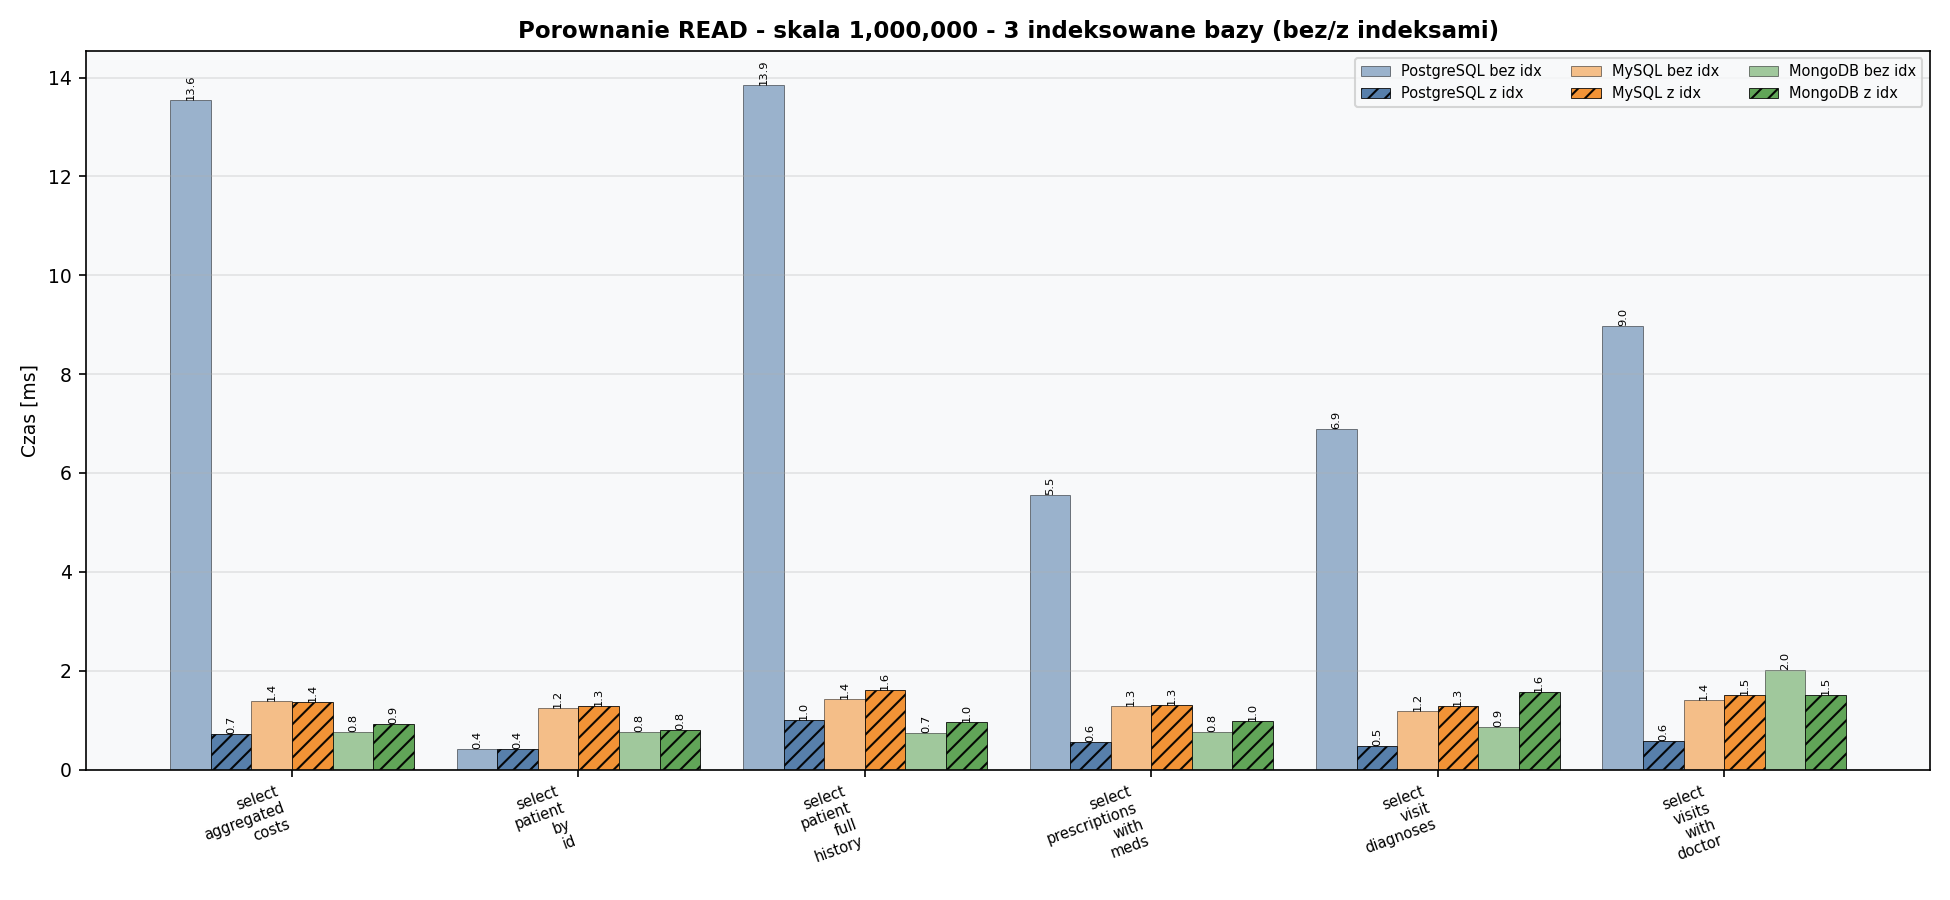
\includegraphics[width=0.95\textwidth]{crud_pair_READ_1000000.png}
\caption{Odczyt danych -- skala 1\,000\,000.}
\label{fig:cp_read_1m}
\end{figure}

\paragraph{Interpretacja wyników.}
Przy 1\,000\,000 rekordów powtarza się ten sam trend, ale bez potrzeby powtarzania całego mechanizmu: PostgreSQL bez indeksów rośnie do około 6--14~ms w~cięższych odczytach, a~po indeksowaniu pozostaje zwykle poniżej 1~ms. MySQL nadal nie pokazuje poprawy wynikającej z~dodatkowych indeksów, a~MongoDB zachowuje się mieszanie: część wyników jest podobna, część nieco gorsza lub lepsza. Odczyt po identyfikatorze pacjenta jest szybki we wszystkich skalach, ponieważ nie wymaga przeszukiwania dużego zbioru rekordów.

\begin{figure}[H]
\centering
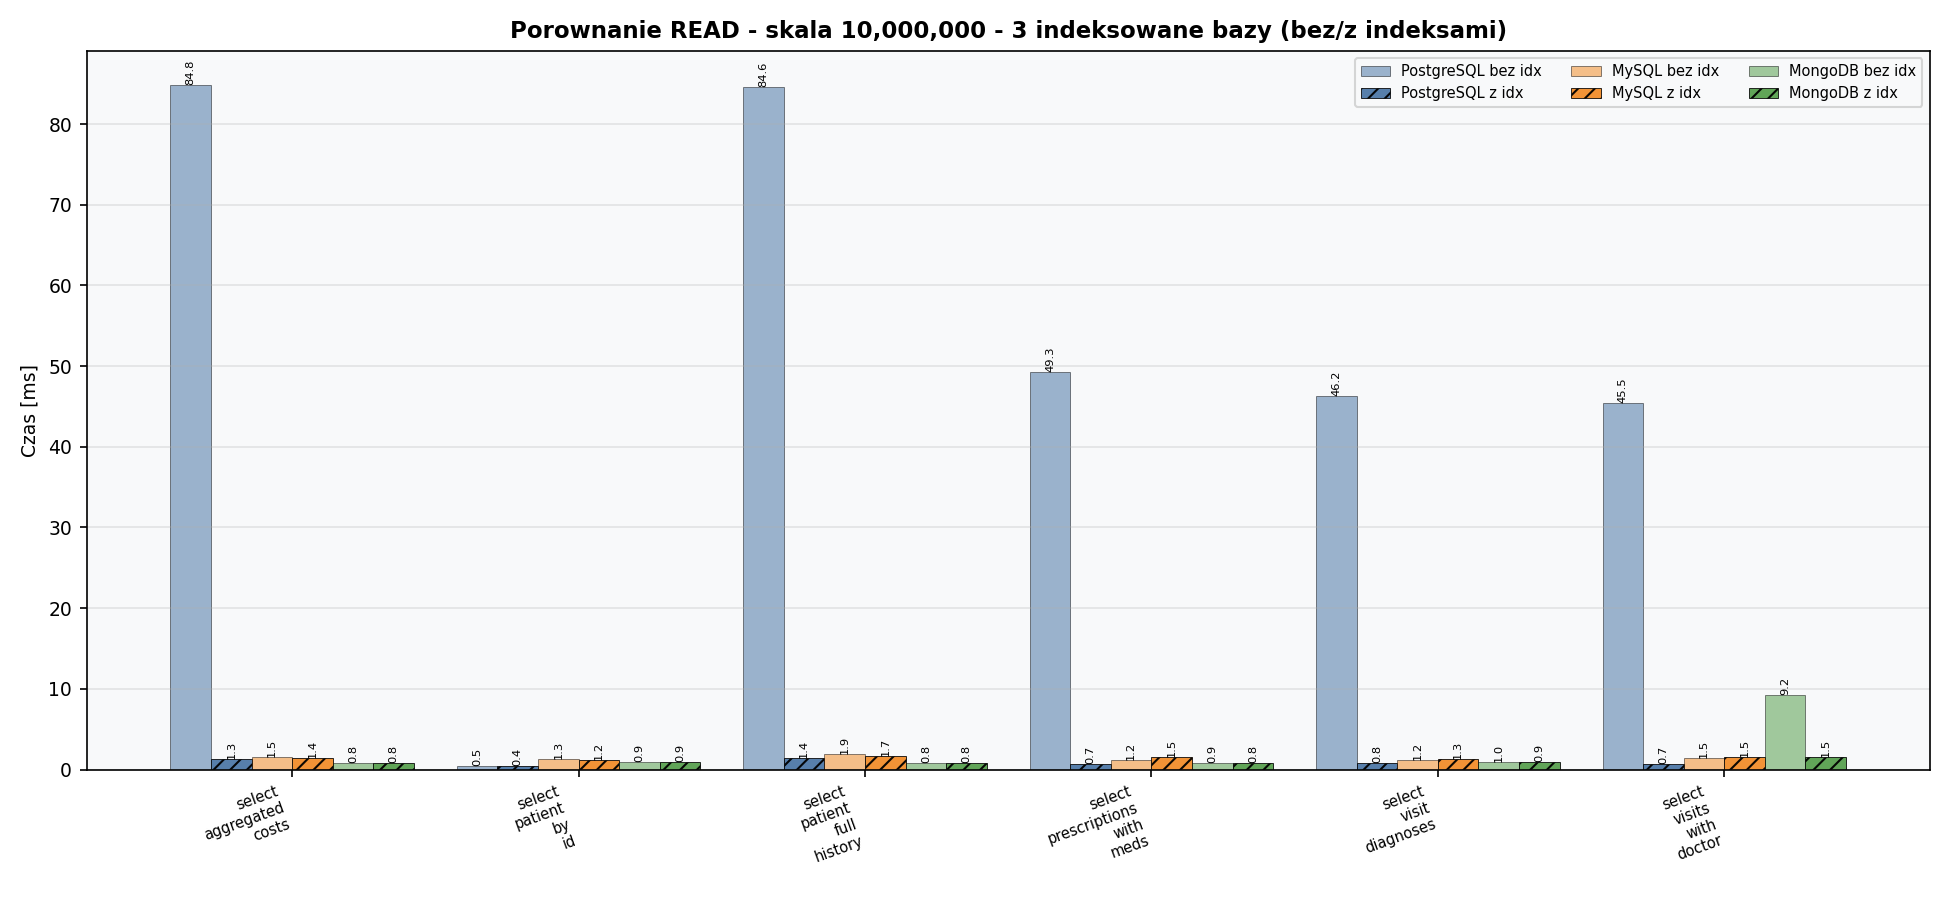
\includegraphics[width=0.95\textwidth]{crud_pair_READ_10000000.png}
\caption{Odczyt danych -- skala 10\,000\,000. PostgreSQL bez indeksów osiąga 45--85~ms, natomiast po zastosowaniu indeksów 0.6--1.5~ms.}
\label{fig:cp_read_10m}
\end{figure}

\paragraph{Interpretacja wyników.}
Na skali 10\,000\,000 rekordów różnice są najbardziej czytelne. PostgreSQL bez indeksów osiąga 45--85~ms w~odczytach zależnych od powiązań, a~po indeksowaniu wraca do około 0.6--1.5~ms. MySQL nadal utrzymuje stabilne, ale nie najlepsze czasy około 1.2--1.7~ms; indeksy dodatkowe nie poprawiają tu wyników w~sposób mierzalny. W~MongoDB znacząca poprawa pojawia się przede wszystkim przy pobraniu wizyt pacjenta z~lekarzem (9.21~ms bez indeksów wobec 1.55~ms z~indeksem). Pozostałe odczyty dokumentowe pozostają szybkie niezależnie od dodatkowych indeksów.

\subsubsection*{Analiza planów wykonania -- odczyt danych}

\textbf{PostgreSQL -- pobranie diagnoz wizyty przy 10M rekordów.} Z~indeksem na identyfikator wizyty w~tabeli diagnoz plan wykorzystuje złączenie haszujące oraz skanowanie indeksu po stronie tabeli diagnoz (4~bloki bufora, czas wykonania \textbf{0.21~ms}). Bez indeksu optymalizator wybiera równoległe sekwencyjne przeszukiwanie tabeli z~2~procesami roboczymi, odczytuje 17\,539~bloków bufora i~filtruje 667\,346 wierszy w~każdym procesie -- czas wykonania wzrasta do \textbf{33.5~ms} (160$\times$ na poziomie planu). Pełny listing znajduje się w~Sekcji~\ref{sec:explain}.

\textbf{PostgreSQL -- wyliczenie sumy kosztów usług przy 500k rekordów.} Z~indeksami silnik wykonuje złączenie pętlowe z~dwoma skanowaniami indeksu (39~bloków bufora, 0.59~ms). Bez indeksów wykorzystuje złączenie haszujące z~dwoma sekwencyjnymi przeglądami tabel (1374 bloki, 13.0~ms). Daje to \textbf{22-krotne przyspieszenie na poziomie planu} dla skali 500k; w~pomiarze właściwym uzyskano $S_{odczyt}=10.79\times$ -- różnica wynika ze stałego narzutu sterownika Python+psycopg, który dominuje nad submilisekundowym planem.

\textbf{MySQL -- pobranie diagnoz wizyty.} Analiza planu pokazuje wyszukanie po indeksie na identyfikatorze wizyty oraz pobranie pojedynczego wiersza po kluczu głównym -- całość trwa 0.01~ms na poziomie silnika. Czas zaobserwowany w~pomiarze właściwym to 1.23~ms, czyli sam silnik odpowiada za około 1\% czasu, a~reszta to protokół klient-serwer i~sterownik. To tłumaczy, dlaczego włączanie lub wyłączanie indeksów w~MySQL nie zmienia istotnie wyniku: różnica między 0.01~ms a~0.5~ms znika przy około 1~ms narzutu komunikacyjnego.

\textbf{MongoDB -- pobranie wizyt pacjenta z~lekarzem.} Z~indeksem na identyfikator lekarza plan wykonuje skanowanie indeksu i~pobranie pasujących dokumentów, badając około 10 dokumentów w~około 1~ms. Bez indeksu silnik wykonuje pełny przegląd kolekcji, badając 2\,000\,000 dokumentów w~około 9~ms. MongoDB nie używa tu równoległości tak jak PostgreSQL, więc skala pełnego przeglądu kolekcji przekłada się bezpośrednio na czas wykonania.

\subsubsection*{Wnioski -- operacje odczytu danych}

\begin{itemize}[noitemsep]
    \item \textbf{Teza o~przyspieszeniu odczytu jest silnie potwierdzona dla PostgreSQL}. Efekt rośnie wraz ze skalą i~przy 10M rekordów osiąga około 59--72-krotność w~scenariuszach opartych na powiązaniach między tabelami.
    \item \textbf{W MySQL dodatkowe indeksy nie dają dużego zysku, ale nie obala to tezy o~znaczeniu indeksów}. W~tym schemacie InnoDB tworzy indeksy wymagane przez klucze obce, więc wariant ,,bez indeksów'' nadal korzysta z~części najważniejszych struktur dostępu. Dlatego czasy odczytu pozostają stabilne, a~różnica między wariantami jest mała.
    \item \textbf{W MongoDB wpływ indeksów jest selektywny}. Wyraźny zysk pojawia się przy pobraniu wizyt pacjenta z~lekarzem na największej skali; odczyty po identyfikatorze dokumentu albo po danych już dobrze osadzonych w~dokumencie pozostają szybkie niezależnie od dodatkowych indeksów.
    \item \textbf{Wniosek praktyczny}: indeksy należy oceniać w~kontekście silnika i~modelu danych. W~PostgreSQL indeksowanie kolumn powiązań jest konieczne dla dużych tabel, w~MySQL efekt może być niewidoczny przy automatycznych indeksach i~dobrym buforowaniu, a~w~MongoDB indeks powinien odpowiadać faktycznemu polu filtrowania.
\end{itemize}

\subsection{Operacja aktualizacji danych}
\label{sec:res_update}

Mierzymy czas pojedynczej aktualizacji danych -- od najprostszej zmiany statusu jednej wizyty po kluczu głównym po aktualizację, w~której warunek filtrowania odnosi się do kolumny klucza obcego i~obejmuje kilka rekordów. Każda wartość to średnia z~3~powtórzeń [ms].

\textbf{Czas wykonania bez indeksów}

\begin{table}[H]
\centering
\caption{Czas operacji aktualizacji danych [ms] -- bez indeksow. Najlepszy wynik w~wierszu pogrubiony.}
\label{tab:update_no}
\small
\begin{tabular}{@{}llrrrr@{}}
\toprule
\textbf{Scenariusz} & \textbf{Skala} & \textbf{PostgreSQL} & \textbf{MySQL} & \textbf{MongoDB} & \textbf{Redis} \\
\midrule
\multirow{3}{*}{\shortstack[l]{Zmiana telefonu\\oddziału}}
 & 500k & 1.18 & 2.86 & 0.80 & \textbf{0.39} \\
 & 1M & 0.94 & 5.40 & 0.76 & \textbf{0.40} \\
 & 10M & 1.06 & 3.99 & 0.75 & \textbf{0.39} \\
\midrule
\multirow{3}{*}{\shortstack[l]{Aktualizacja notatek\\diagnozy}}
 & 500k & 4.58 & 2.14 & \textbf{0.82} & 1.03 \\
 & 1M & 7.10 & 3.72 & \textbf{0.72} & 0.81 \\
 & 10M & 97.07 & 2.80 & \textbf{0.71} & 0.82 \\
\midrule
\multirow{3}{*}{\shortstack[l]{Zmiana licencji\\lekarza}}
 & 500k & 1.32 & 4.49 & 2.39 & \textbf{0.42} \\
 & 1M & 0.94 & 4.96 & 0.75 & \textbf{0.41} \\
 & 10M & 1.14 & 3.91 & 0.81 & \textbf{0.39} \\
\midrule
\multirow{3}{*}{\shortstack[l]{Zmiana nazwiska\\pacjenta}}
 & 500k & 1.13 & 3.46 & 0.76 & \textbf{0.44} \\
 & 1M & 1.09 & 3.89 & 0.75 & \textbf{0.44} \\
 & 10M & 1.07 & 3.90 & 0.79 & \textbf{0.44} \\
\midrule
\multirow{3}{*}{\shortstack[l]{Zmiana ceny\\wykonanej usługi}}
 & 500k & 4.08 & 2.67 & 0.73 & \textbf{0.48} \\
 & 1M & 7.05 & 6.01 & 0.71 & \textbf{0.47} \\
 & 10M & 67.45 & 5.37 & 0.71 & \textbf{0.41} \\
\midrule
\multirow{3}{*}{\shortstack[l]{Zmiana statusu\\wizyty}}
 & 500k & 1.19 & 3.83 & 0.72 & \textbf{0.51} \\
 & 1M & 0.94 & 2.07 & 0.72 & \textbf{0.38} \\
 & 10M & 1.03 & 2.06 & \textbf{0.69} & 0.83 \\
\bottomrule
\end{tabular}
\end{table}


\textbf{Czas wykonania z~indeksami}

\begin{table}[H]
\centering
\caption{Czas operacji aktualizacji danych [ms] -- z~indeksami. Najlepszy wynik w~wierszu pogrubiony. Redis nie posiada mechanizmu indeksow (kolumna `---').}
\label{tab:update_idx}
\small
\begin{tabular}{@{}llrrrr@{}}
\toprule
\textbf{Scenariusz} & \textbf{Skala} & \textbf{PostgreSQL} & \textbf{MySQL} & \textbf{MongoDB} & \textbf{Redis} \\
\midrule
\multirow{3}{*}{\shortstack[l]{Zmiana telefonu\\oddziału}}
 & 500k & 1.02 & 3.78 & \textbf{0.75} & --- \\
 & 1M & 1.25 & 4.74 & \textbf{0.71} & --- \\
 & 10M & \textbf{1.29} & 4.05 & 1.47 & --- \\
\midrule
\multirow{3}{*}{\shortstack[l]{Aktualizacja notatek\\diagnozy}}
 & 500k & 1.08 & 3.85 & \textbf{0.76} & --- \\
 & 1M & 1.03 & 2.24 & \textbf{0.72} & --- \\
 & 10M & 1.54 & 2.45 & \textbf{0.74} & --- \\
\midrule
\multirow{3}{*}{\shortstack[l]{Zmiana licencji\\lekarza}}
 & 500k & 1.38 & 4.49 & \textbf{0.77} & --- \\
 & 1M & 1.00 & 3.99 & \textbf{0.82} & --- \\
 & 10M & 1.09 & 3.40 & \textbf{0.76} & --- \\
\midrule
\multirow{3}{*}{\shortstack[l]{Zmiana nazwiska\\pacjenta}}
 & 500k & 1.21 & 4.21 & \textbf{0.76} & --- \\
 & 1M & 1.03 & 4.43 & \textbf{0.84} & --- \\
 & 10M & 1.50 & 4.74 & \textbf{0.89} & --- \\
\midrule
\multirow{3}{*}{\shortstack[l]{Zmiana ceny\\wykonanej usługi}}
 & 500k & \textbf{0.45} & 4.11 & 0.78 & --- \\
 & 1M & \textbf{0.63} & 3.54 & 0.72 & --- \\
 & 10M & 0.94 & 4.28 & \textbf{0.74} & --- \\
\midrule
\multirow{3}{*}{\shortstack[l]{Zmiana statusu\\wizyty}}
 & 500k & 1.11 & 4.25 & \textbf{0.71} & --- \\
 & 1M & 0.99 & 3.23 & \textbf{0.77} & --- \\
 & 10M & 1.28 & 3.44 & \textbf{0.80} & --- \\
\bottomrule
\end{tabular}
\end{table}


\subsubsection*{Porównanie baz na trzech skalach}

\begin{figure}[H]
\centering
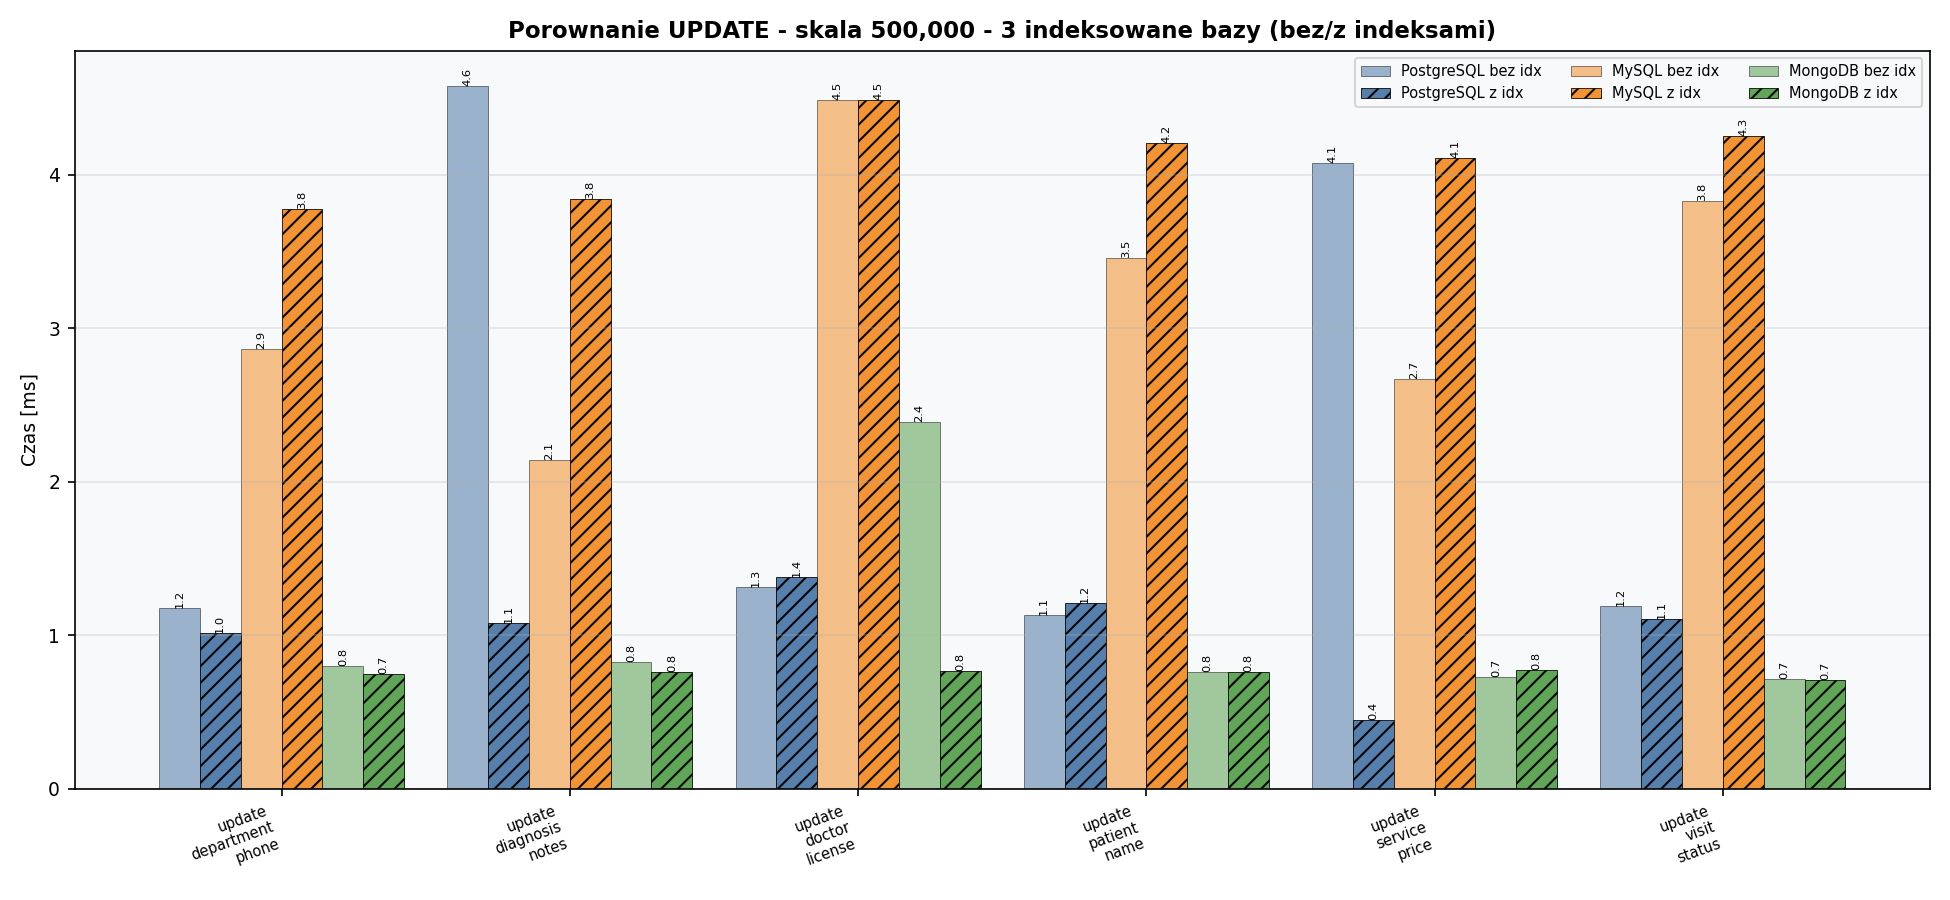
\includegraphics[width=0.95\textwidth]{crud_pair_UPDATE_500000.png}
\caption{Aktualizacja danych -- skala 500\,000.}
\label{fig:cp_update_500k}
\end{figure}

\paragraph{Interpretacja wyników.}
Na skali 500\,000 rekordów większość aktualizacji mieści się w~kilku milisekundach. MongoDB jest zwykle najszybsza, MySQL ma wyraźnie wyższy koszt zapisu, a~PostgreSQL zachowuje się dwojako. Przy zmianie ceny wykonanej usługi i~aktualizacji notatek diagnozy indeksy obniżają czas z~około 4--5~ms do około 1~ms, ponieważ pomagają znaleźć rekordy powiązane z~wizytą. W~aktualizacjach po identyfikatorze, takich jak zmiana nazwiska pacjenta lub statusu wizyty, zysk z~wyszukiwania już istnieje dzięki kluczowi głównemu, więc dodatkowe indeksy mogą być wyłącznie narzutem.

\begin{figure}[H]
\centering
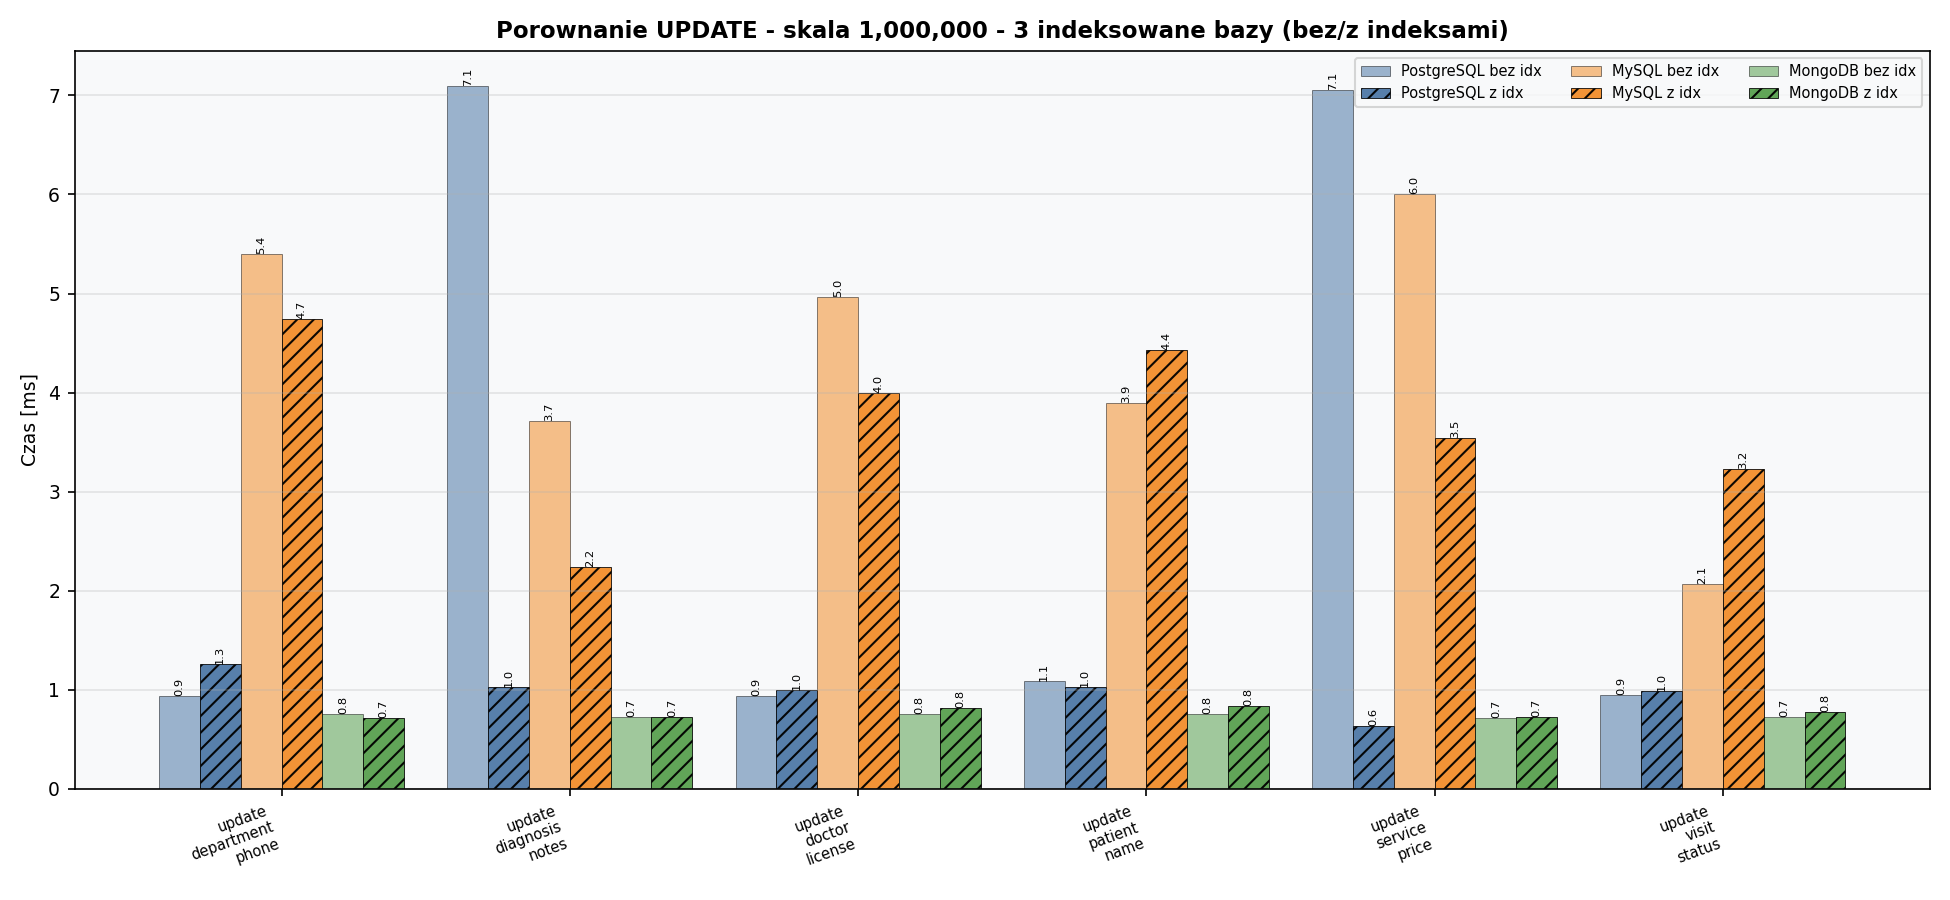
\includegraphics[width=0.95\textwidth]{crud_pair_UPDATE_1000000.png}
\caption{Aktualizacja danych -- skala 1\,000\,000.}
\label{fig:cp_update_1m}
\end{figure}

\paragraph{Interpretacja wyników.}
Przy 1\,000\,000 rekordów nie pojawia się nowy mechanizm, tylko pogłębia się różnica w~PostgreSQL dla aktualizacji wyszukujących dane po kolumnie powiązania: bez indeksów czas rośnie do około 7~ms, a~z~indeksami pozostaje blisko 0.6--1.0~ms. MySQL i~MongoDB nie pokazują takiej zależności od skali; ich wyniki są raczej stabilne albo mieszane, co wskazuje, że w~tych silnikach koszt pojedynczej aktualizacji jest w~tym teście zdominowany przez inne elementy niż sam rozmiar zbioru.

\begin{figure}[H]
\centering
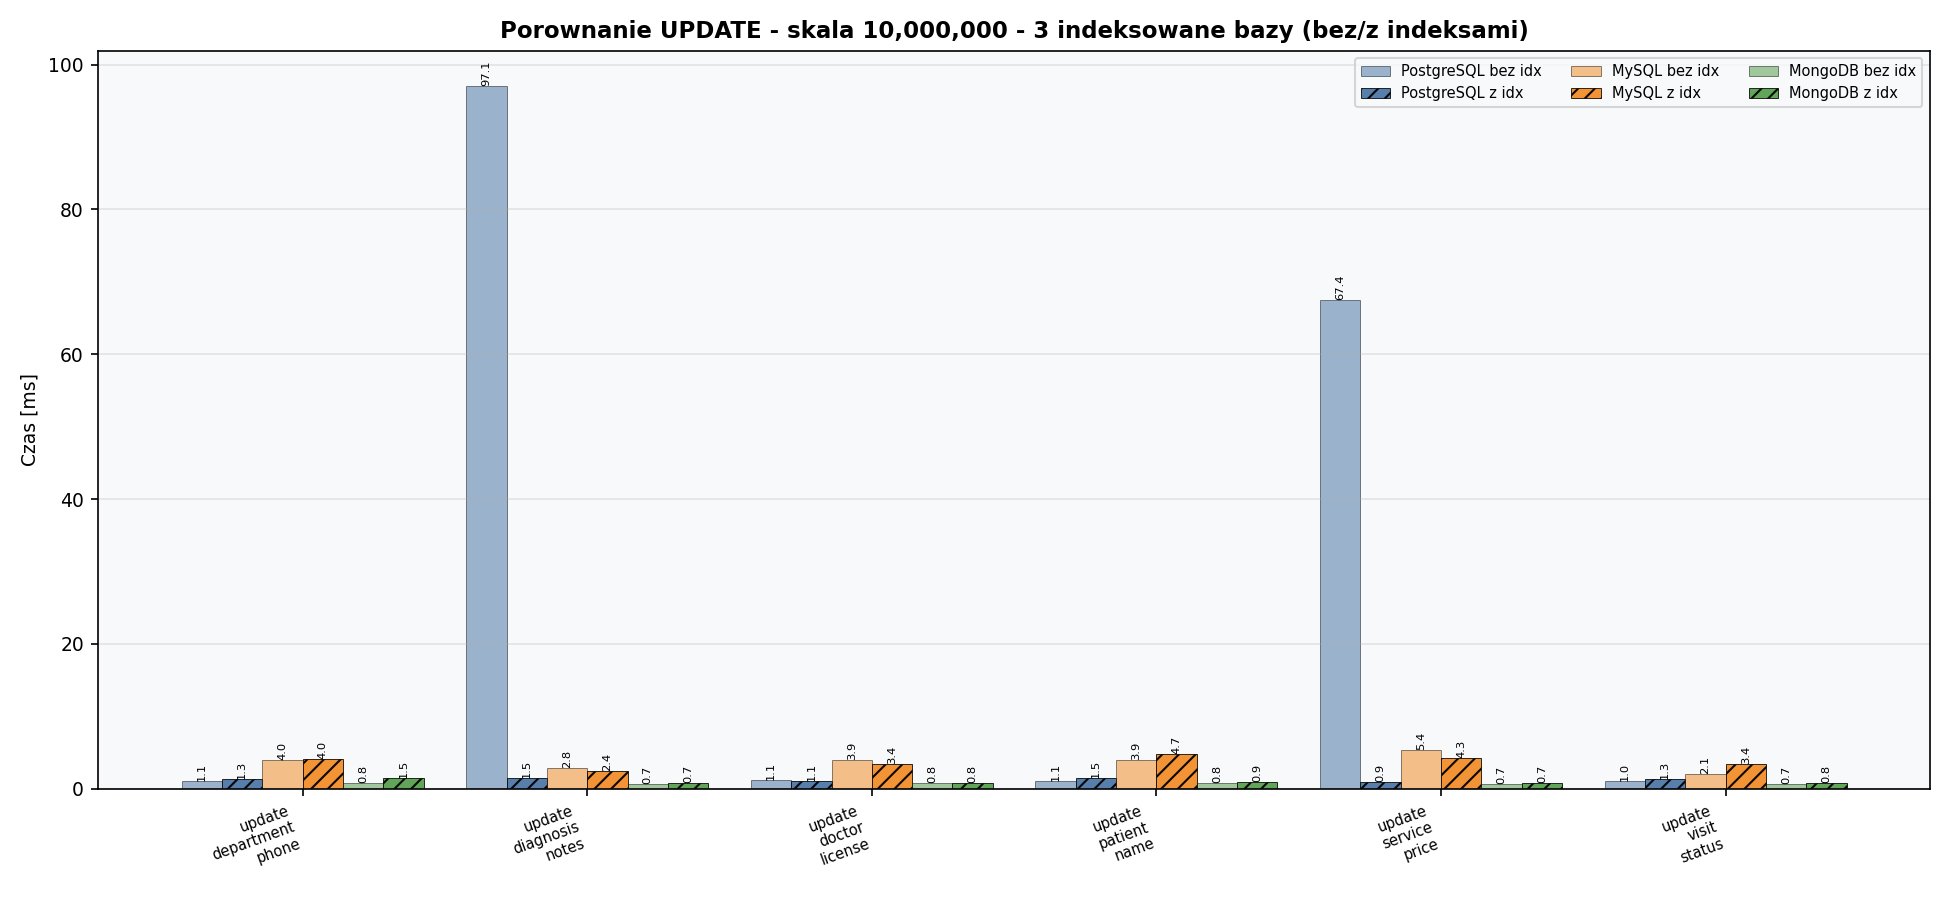
\includegraphics[width=0.95\textwidth]{crud_pair_UPDATE_10000000.png}
\caption{Aktualizacja danych -- skala 10\,000\,000. PostgreSQL bez indeksów dla zmiany ceny wykonanej usługi i~aktualizacji notatek diagnozy osiąga 67--97~ms.}
\label{fig:cp_update_10m}
\end{figure}

\paragraph{Interpretacja wyników.}
Na skali 10\,000\,000 rekordów różnica w~PostgreSQL staje się bardzo duża: zmiana ceny wykonanej usługi oraz aktualizacja notatek diagnozy bez indeksów osiągają 67--97~ms, a~z~indeksami około 1~ms. Nie oznacza to, że indeksy zawsze przyspieszają zapis; oznacza to, że w~tych dwóch scenariuszach koszt znalezienia rekordów jest większy niż koszt samej modyfikacji. Jednocześnie zmiana statusu wizyty w~PostgreSQL zwalnia po dodaniu indeksów z~1.03 do 1.28~ms, a~w~MySQL z~2.06 do 3.44~ms. Tabele pokazują więc dwa zjawiska naraz: indeks może dramatycznie pomóc, gdy jest potrzebny do znalezienia rekordów, ale może spowolnić aktualizację po kluczu głównym.

\subsubsection*{Analiza planów wykonania -- aktualizacja danych}

\textbf{PostgreSQL -- zmiana ceny wykonanej usługi przy 10M rekordów.} Z~indeksem na identyfikator wizyty w~tabeli wykonanych usług plan aktualizacji poprzedzony jest skanowaniem indeksu (4~bloki bufora, czas wykonania \textbf{0.09~ms}). Bez indeksu silnik wykonuje sekwencyjne przeszukiwanie tabeli z~filtrem po identyfikatorze wizyty, odrzucając 2\,000\,195 wierszy (12\,741~bloków bufora, czas wykonania \textbf{63.0~ms}). To około 700-krotne przyspieszenie na poziomie planu i~tłumaczy bezpośrednio, dlaczego $K_{zapis}=0.02$ dla tego scenariusza -- koszt wyszukania kilku wierszy do aktualizacji \emph{dominuje} nad narzutem aktualizacji indeksów, więc dodanie indeksów daje netto przyspieszenie zapisu.

\textbf{PostgreSQL -- zmiana statusu wizyty.} Tu plan wygląda identycznie z~i~bez indeksów dodatkowych: aktualizacja wizyty poprzedzona jest skanowaniem indeksu po kluczu głównym tabeli wizyt (jednoznaczny dostęp, $<$0.1~ms). Różnicę robi tylko narzut aktualizacji indeksów wtórnych -- przy każdej aktualizacji wiersza trzeba przepisać wpisy w~dodatkowych indeksach dotyczących lekarza, statusu, daty wizyty itp. Stąd wariant ,,z~indeksami'' jest około 24\% wolniejszy.

\textbf{MySQL -- zmiana statusu wizyty.} Interpretacja jest taka sama jak w~PostgreSQL, ale efekt jest silniejszy ($+67\%$ przy 10M) -- każdy zapis musi dodatkowo zaktualizować dziennik odtwarzania i~dziennik binarny oraz wymusić synchronizację dyskową, więc każdy dodatkowy indeks dokłada koszt nie tylko aktualizacji struktury indeksu, ale też wpisu do dziennika.

\subsubsection*{Wnioski -- operacje aktualizacji danych}

\begin{itemize}[noitemsep]
    \item \textbf{Aktualizacje nie potwierdzają prostej wersji hipotezy}. Nie można powiedzieć, że indeksy po prostu spowalniają zapis: w~PostgreSQL dla aktualizacji po kolumnie powiązania indeksy przyspieszają operację kilkadziesiąt razy.
    \item \textbf{Spowolnienie zapisu jest widoczne tam, gdzie rekord i~tak jest odnajdywany po kluczu głównym}. Przykładem jest zmiana statusu wizyty: przy 10M rekordów PostgreSQL zwalnia o~około 24\%, a~MySQL o~około 67\%.
    \item \textbf{MySQL ma stabilne, ale relatywnie wysokie czasy aktualizacji}. Wynika to z~kosztu trwałego zatwierdzania zmian; dodatkowe indeksy często zwiększają koszt, choć nie w~każdym scenariuszu tak samo.
    \item \textbf{MongoDB osiąga najniższe czasy aktualizacji} spośród baz biorących udział w~badaniu indeksów, ponieważ operuje głównie po identyfikatorach dokumentów. Dodatkowe indeksy nie tworzą tu silnego, regularnego trendu.
    \item \textbf{Wniosek praktyczny}: indeksuj kolumny używane do wyszukania aktualizowanych rekordów, ale nie traktuj każdego indeksu jako darmowego. Jeżeli aktualizacja dotyczy często zmienianej kolumny i~rekord jest już odnajdywany po kluczu głównym, dodatkowy indeks może być czystym kosztem.
\end{itemize}

\subsection{Operacja usuwania danych}
\label{sec:res_delete}

Mierzymy czas pojedynczej operacji usuwania danych -- od prostych ,,liści'', takich jak usunięcie wyniku badania bez rekordów potomnych, po kaskadowe usunięcie wizyty wraz z~jej diagnozami, usługami, lekami i~innymi powiązanymi rekordami. Każda wartość to średnia z~3~powtórzeń [ms].

\textbf{Czas wykonania bez indeksów}

\begin{table}[H]
\centering
\caption{Czas operacji usuwania danych [ms] -- bez indeksow. Najlepszy wynik w~wierszu pogrubiony.}
\label{tab:delete_no}
\small
\begin{tabular}{@{}llrrrr@{}}
\toprule
\textbf{Scenariusz} & \textbf{Skala} & \textbf{PostgreSQL} & \textbf{MySQL} & \textbf{MongoDB} & \textbf{Redis} \\
\midrule
\multirow{3}{*}{\shortstack[l]{Usunięcie\\diagnozy}}
 & 500k & 0.95 & 4.65 & 0.74 & \textbf{0.43} \\
 & 1M & 0.93 & 3.84 & 0.70 & \textbf{0.39} \\
 & 10M & 1.13 & 4.45 & 0.71 & \textbf{0.40} \\
\midrule
\multirow{3}{*}{\shortstack[l]{Usunięcie\\pacjenta}}
 & 500k & 4.64 & 5.01 & 0.69 & \textbf{0.50} \\
 & 1M & 7.52 & 3.80 & 0.82 & \textbf{0.49} \\
 & 10M & 78.57 & 4.05 & 0.69 & \textbf{0.39} \\
\midrule
\multirow{3}{*}{\shortstack[l]{Usunięcie\\wykonanej usługi}}
 & 500k & 1.07 & 4.90 & 0.76 & \textbf{0.43} \\
 & 1M & 0.98 & 4.26 & 0.72 & \textbf{0.38} \\
 & 10M & 1.09 & 3.84 & 0.72 & \textbf{0.38} \\
\midrule
\multirow{3}{*}{\shortstack[l]{Usunięcie\\recepty}}
 & 500k & 3.66 & 4.60 & 0.73 & \textbf{0.51} \\
 & 1M & 6.24 & 4.09 & 0.82 & \textbf{0.38} \\
 & 10M & 61.49 & 4.47 & 0.76 & \textbf{0.38} \\
\midrule
\multirow{3}{*}{\shortstack[l]{Usunięcie\\wyniku badania}}
 & 500k & 1.02 & 4.34 & 0.74 & \textbf{0.44} \\
 & 1M & 0.93 & 4.19 & 0.73 & \textbf{0.39} \\
 & 10M & 1.07 & 4.06 & 0.71 & \textbf{0.40} \\
\midrule
\multirow{3}{*}{\shortstack[l]{Kaskadowe\\usunięcie wizyty}}
 & 500k & 12.75 & 12.29 & 0.73 & \textbf{0.59} \\
 & 1M & 22.79 & 4.05 & 0.84 & \textbf{0.39} \\
 & 10M & 224.6 & 4.23 & 0.73 & \textbf{0.42} \\
\bottomrule
\end{tabular}
\end{table}


\textbf{Czas wykonania z~indeksami}

\begin{table}[H]
\centering
\caption{Czas operacji usuwania danych [ms] -- z~indeksami. Najlepszy wynik w~wierszu pogrubiony. Redis nie posiada mechanizmu indeksow (kolumna `---').}
\label{tab:delete_idx}
\small
\begin{tabular}{@{}llrrrr@{}}
\toprule
\textbf{Scenariusz} & \textbf{Skala} & \textbf{PostgreSQL} & \textbf{MySQL} & \textbf{MongoDB} & \textbf{Redis} \\
\midrule
\multirow{3}{*}{\shortstack[l]{Usunięcie\\diagnozy}}
 & 500k & 1.01 & 5.10 & \textbf{0.76} & --- \\
 & 1M & 0.95 & 4.24 & \textbf{0.74} & --- \\
 & 10M & 0.99 & 4.02 & \textbf{0.80} & --- \\
\midrule
\multirow{3}{*}{\shortstack[l]{Usunięcie\\pacjenta}}
 & 500k & 1.04 & 4.51 & \textbf{0.72} & --- \\
 & 1M & 1.06 & 3.86 & \textbf{0.73} & --- \\
 & 10M & 1.03 & 3.82 & \textbf{0.71} & --- \\
\midrule
\multirow{3}{*}{\shortstack[l]{Usunięcie\\wykonanej usługi}}
 & 500k & 0.98 & 4.18 & \textbf{0.81} & --- \\
 & 1M & 0.94 & 3.97 & \textbf{0.78} & --- \\
 & 10M & 1.02 & 4.12 & \textbf{0.71} & --- \\
\midrule
\multirow{3}{*}{\shortstack[l]{Usunięcie\\recepty}}
 & 500k & 1.13 & 4.04 & \textbf{0.71} & --- \\
 & 1M & 0.98 & 4.47 & \textbf{0.72} & --- \\
 & 10M & 1.00 & 3.91 & \textbf{0.73} & --- \\
\midrule
\multirow{3}{*}{\shortstack[l]{Usunięcie\\wyniku badania}}
 & 500k & 0.99 & 3.73 & \textbf{0.76} & --- \\
 & 1M & 1.25 & 3.99 & \textbf{0.69} & --- \\
 & 10M & 1.06 & 4.13 & \textbf{0.71} & --- \\
\midrule
\multirow{3}{*}{\shortstack[l]{Kaskadowe\\usunięcie wizyty}}
 & 500k & 1.08 & 4.50 & \textbf{0.78} & --- \\
 & 1M & 1.01 & 4.53 & \textbf{0.77} & --- \\
 & 10M & 1.05 & 4.43 & \textbf{0.80} & --- \\
\bottomrule
\end{tabular}
\end{table}


\subsubsection*{Porównanie baz na trzech skalach}

\begin{figure}[H]
\centering
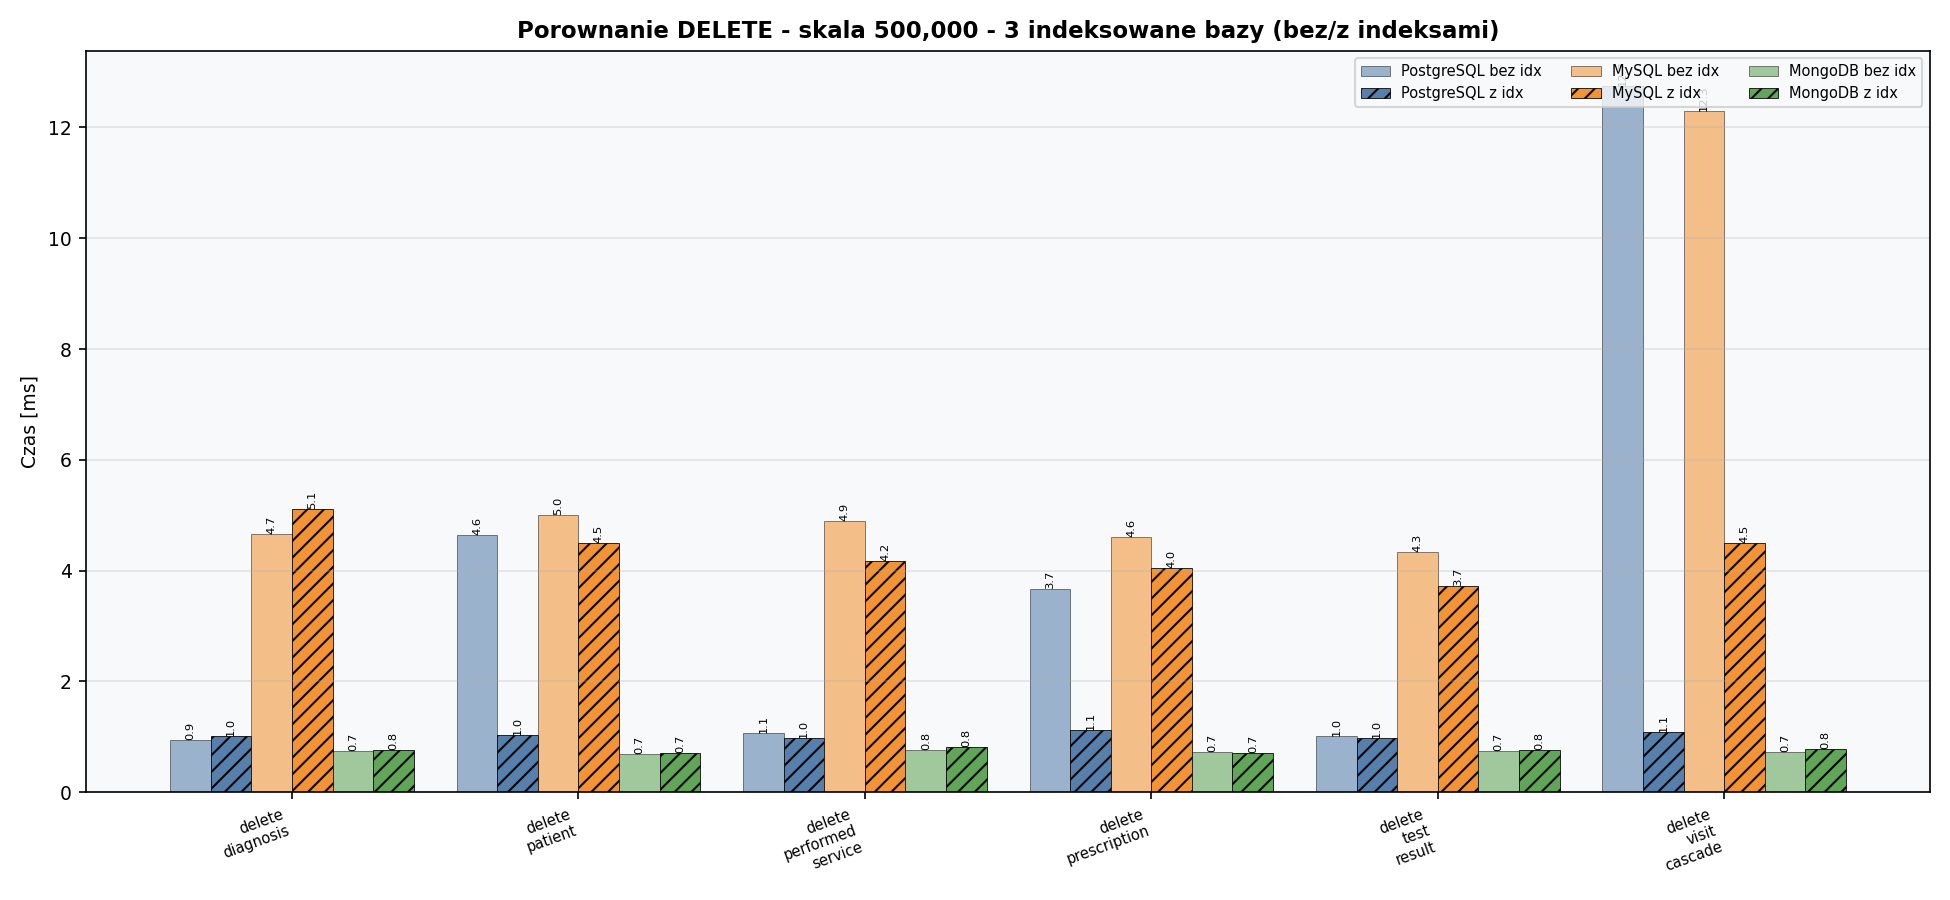
\includegraphics[width=0.95\textwidth]{crud_pair_DELETE_500000.png}
\caption{Usuwanie danych -- skala 500\,000.}
\label{fig:cp_delete_500k}
\end{figure}

\paragraph{Interpretacja wyników.}
Na skali 500\,000 rekordów usuwanie rekordów bez zależnych danych pozostaje krótkie we wszystkich bazach, szczególnie w~MongoDB. Różnica pojawia się przy usuwaniu rekordów nadrzędnych, czyli pacjenta, recepty i~wizyty. W~PostgreSQL bez indeksów kaskadowe usunięcie wizyty trwa około 13~ms, a~po indeksowaniu około 1~ms. MySQL ma przy tej skali również wysoki wynik dla kaskadowego usunięcia wizyty bez dodatkowych indeksów, lecz w~kolejnych skalach utrzymuje się blisko 4~ms dzięki indeksom wymaganym przez mechanizmy integralności.

\begin{figure}[H]
\centering
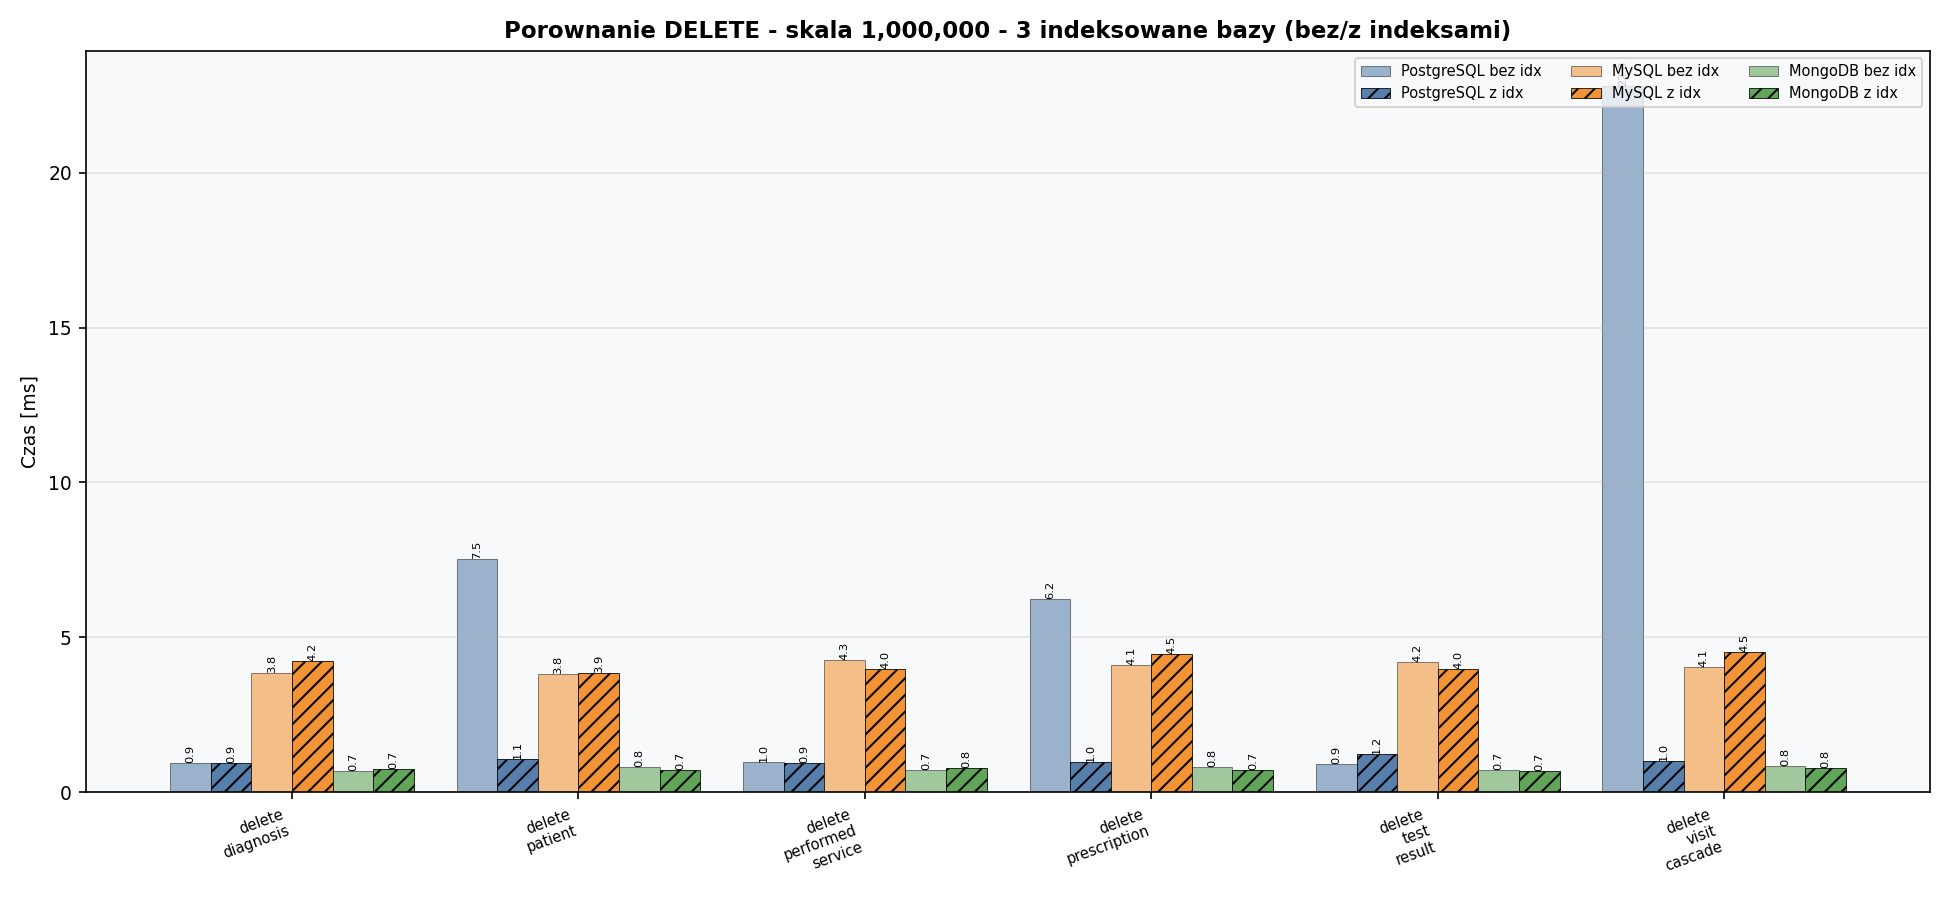
\includegraphics[width=0.95\textwidth]{crud_pair_DELETE_1000000.png}
\caption{Usuwanie danych -- skala 1\,000\,000.}
\label{fig:cp_delete_1m}
\end{figure}

\paragraph{Interpretacja wyników.}
Przy 1\,000\,000 rekordów wzorzec jest analogiczny: w~PostgreSQL bez indeksów rosną przede wszystkim usunięcia rekordów mających zależności, szczególnie wizyta, pacjent i~recepta. Po indeksowaniu wszystkie te przypadki wracają w~okolice 1~ms. Usunięcia pojedynczych rekordów bez potomków pozostają stabilne, więc problemem nie jest samo usunięcie wiersza, lecz konieczność odnalezienia powiązanych rekordów w~tabelach zależnych.

\begin{figure}[H]
\centering
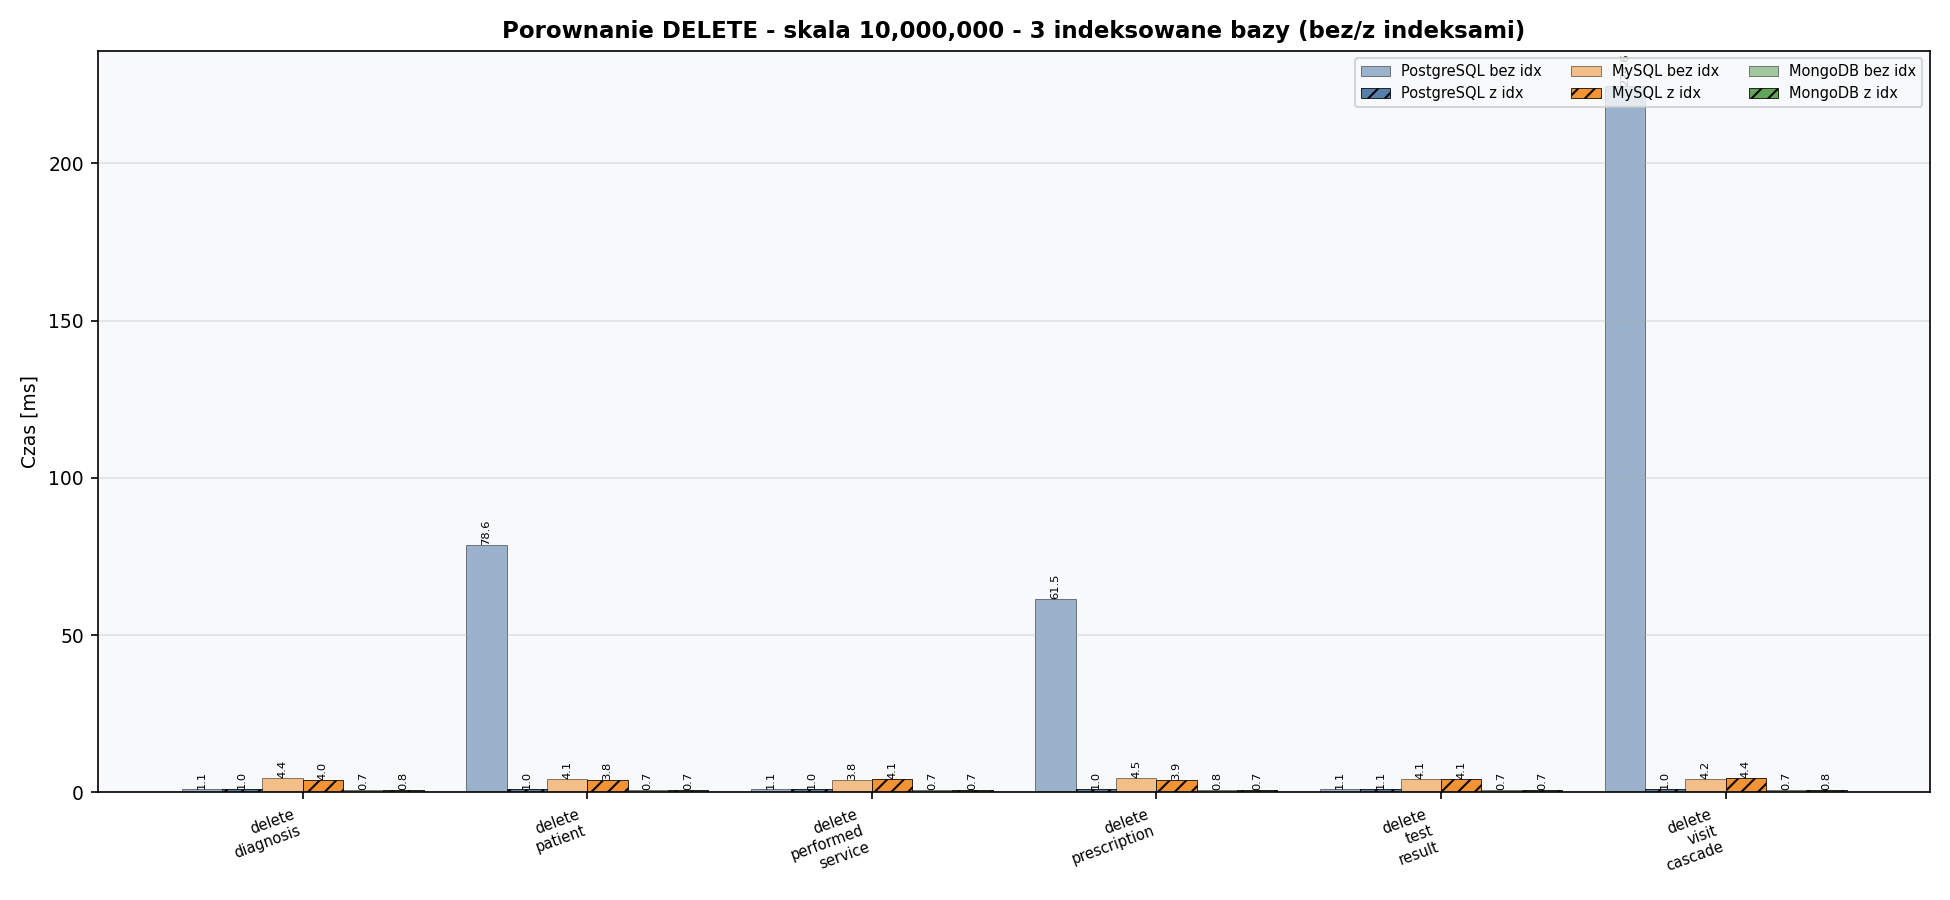
\includegraphics[width=0.95\textwidth]{crud_pair_DELETE_10000000.png}
\caption{Usuwanie danych -- skala 10\,000\,000. PostgreSQL bez indeksów dla kaskadowego usunięcia wizyty osiąga 225~ms; z~indeksami spada do 1~ms.}
\label{fig:cp_delete_10m}
\end{figure}

\paragraph{Interpretacja wyników.}
Na skali 10\,000\,000 rekordów kaskadowe usunięcie wizyty w~PostgreSQL bez indeksów osiąga około 225~ms, a~z~indeksami około 1~ms. Podobny, choć mniejszy, efekt dotyczy usunięcia pacjenta i~recepty. Dla rekordów bez potomków indeksy nie zmieniają wyniku istotnie, bo wystarcza dostęp po kluczu głównym. W~MySQL czasy usuwania pozostają blisko 4~ms, a~MongoDB utrzymuje około 0.7--0.8~ms, dlatego wniosek o~krytycznym znaczeniu indeksów dotyczy tu przede wszystkim PostgreSQL i~operacji na rekordach nadrzędnych.

\subsubsection*{Analiza planów wykonania -- usuwanie danych}

\textbf{PostgreSQL -- kaskadowe usunięcie wizyty przy 10M rekordów.} Z~indeksami plan obejmuje usunięcie wizyty po kluczu głównym oraz sześć usunięć w~tabelach potomnych z~wyszukaniem przez indeks po kolumnie klucza obcego. Łączny czas wykonania wynosi \textbf{1.05~ms}. Bez indeksów PostgreSQL nadal odnajduje wizytę po kluczu głównym w~czasie poniżej 0.1~ms, ale kaskadowe usuwanie wymaga wyszukania potomków -- każda z~6~tabel jest skanowana sekwencyjnie po 2--10~mln wierszy. Pojedynczy sekwencyjny przegląd tabeli wykonanych usług (2~mln wierszy) trwa około 35~ms, więc 6~takich skanów sumarycznie daje około \textbf{225~ms}. To około 215-krotne przyspieszenie, największe w~całym pomiarze.

\textbf{PostgreSQL -- usuwanie rekordów bez potomków.} Dla usunięcia wyniku badania, diagnozy lub wykonanej usługi plan jest prosty: usunięcie z~tabeli po wyszukaniu wiersza przez klucz główny w~czasie około 0.05~ms. Brak potomków oznacza brak dodatkowych skanów. Dodatkowe indeksy nie zmieniają czasu wyszukania, ponieważ klucz główny i~tak istnieje, więc ich obecność tworzy tylko niewielki narzut na usunięcie wpisów.

\textbf{MySQL.} Kaskadowe usunięcie wizyty korzysta z~automatycznych indeksów wymuszonych przez klucze obce -- plan wykonuje usunięcie z~wyszukaniem po indeksie dla każdej tabeli potomnej. Czasy są stabilne i~wynoszą około 4~ms w~obu wariantach, ponieważ kluczowe indeksy są zawsze obecne.

\textbf{MongoDB.} Wszystkie usunięcia dotyczą pojedynczego dokumentu wyszukiwanego po identyfikatorze, więc plan korzysta z~najszybszej ścieżki dostępu po kluczu dokumentu. Brak kaskady w~silniku oznacza brak dodatkowych skanów.

\subsubsection*{Wnioski -- operacje usuwania danych}

\begin{itemize}[noitemsep]
    \item \textbf{Największy efekt indeksów w~całym pomiarze dotyczy PostgreSQL i~usuwania rekordów nadrzędnych}. Kaskadowe usunięcie wizyty przy 10M rekordów skraca się z~224.62 do 1.04~ms, czyli około 215-krotnie.
    \item \textbf{Indeksy nie są równie ważne dla każdego usunięcia}. Wynik badania, diagnoza i~wykonana usługa są usuwane szybko niezależnie od wariantu, ponieważ nie wymagają sprawdzania dużych tabel potomnych.
    \item \textbf{MySQL i~MongoDB nie pokazują takiego samego efektu jak PostgreSQL}. MySQL korzysta z~indeksów wymaganych przez integralność relacyjną, a~MongoDB usuwa pojedyncze dokumenty po identyfikatorze; dlatego ich czasy są stabilniejsze między skalami.
    \item \textbf{Wniosek praktyczny}: w~PostgreSQL kolumny kluczy obcych używane przy usuwaniu kaskadowym muszą być indeksowane ręcznie. W~przeciwnym razie usunięcie jednego rekordu nadrzędnego może wymusić wielokrotne przeglądanie wielomilionowych tabel zależnych.
\end{itemize}


% ══════════════════════════════════════════════════════════════════════
\section{Analiza indeksów}
% ══════════════════════════════════════════════════════════════════════

\subsection{Zastosowane indeksy}

W~systemach relacyjnych utworzono 16 indeksów B-tree na kolumnach kluczy obcych i~kolumnach filtrujących. W~MongoDB utworzono 7~indeksów na kolekcji pacjentów, m.in. dla statusu wizyty, identyfikatora lekarza oraz identyfikatora choroby w~zagnieżdżonej diagnozie.

\subsection{Analiza planów wykonania zapytań}
\label{sec:explain}

W~celu uwiarygodnienia interpretacji wyników pomiaru wykonano dodatkowe analizy planów wykonania zapytań w~PostgreSQL, MySQL i~MongoDB. Pełne wyniki znajdują się w~katalogu \texttt{results}.

\subsubsection{PostgreSQL -- pobranie diagnoz wizyty (10M, złączenie po kluczu obcym)}

\textbf{Z indeksami}:
\begin{lstlisting}[basicstyle=\ttfamily\scriptsize]
Hash Join  (cost=8.49..21.01 rows=2 width=53) (actual time=0.151..0.153 rows=0)
  Buffers: shared hit=1 read=3
  -> Seq Scan on diseases ds  (rows=1)
  -> Hash -> Index Scan using idx_diagnoses_visit_id on diagnoses dg
        Index Cond: (visit_id = 1)
        Buffers: shared read=3
Planning Time: 1.221 ms;  Execution Time: 0.208 ms
\end{lstlisting}

\textbf{Bez indeksów}:
\begin{lstlisting}[basicstyle=\ttfamily\scriptsize]
Gather  (cost=1000.28..28974.80 rows=2) (actual time=29.111..33.436)
  Workers Planned: 2;  Workers Launched: 2
  Buffers: shared hit=17539
  -> Parallel Seq Scan on diagnoses dg
        Filter: (visit_id = 1);  Rows Removed by Filter: 667346
        Buffers: shared hit=17539
Execution Time: 33.454 ms
\end{lstlisting}

Dla 2~mln diagnoz przy 10M sumarycznych rekordów optymalizator wybiera równoległe sekwencyjne przeszukiwanie tabeli z~2~procesami roboczymi (17\,539 trafień w~buforze) zamiast zwykłego sekwencyjnego przeglądu. Mimo zrównoleglenia czas wzrasta z~0.2~ms do 33.5~ms ($\approx$160$\times$ w~planie; w~pomiarze właściwym 88$\times$ ze względu na stały narzut Python+psycopg na pojedynczy pomiar).

\subsubsection{PostgreSQL -- wyliczenie sumy kosztów usług (500k, kontrolna analiza planu)}
\label{sec:explain_500k}

\textbf{Z indeksami}:
\begin{lstlisting}[basicstyle=\ttfamily\scriptsize]
Limit  (actual time=... rows=8)
  -> GroupAggregate -> Sort -> Nested Loop
      -> Index Scan using idx_visits_patient_id on visits v
            Index Cond: (patient_id = ?);  rows=12
      -> Index Scan using idx_performed_services_visit_id on ps
            Index Cond: (visit_id = v.id);  rows=1, loops=12
  Buffers: shared hit=27 read=12
Execution Time: 0.588 ms
\end{lstlisting}

\textbf{Bez indeksów}:
\begin{lstlisting}[basicstyle=\ttfamily\scriptsize]
Limit  (actual time=... rows=8)
  -> Hash Join
      Hash Cond: (ps.visit_id = v.id)
      -> Seq Scan on performed_services ps  (rows=100119)
      -> Hash -> Seq Scan on visits v
            Filter: (patient_id = ?);  Rows Removed by Filter: 99989
  Buffers: shared hit=1374
Execution Time: 13.005 ms
\end{lstlisting}

\textbf{Wniosek}: kontrolna analiza planu na skali 500k pokazuje \textbf{22-krotne przyspieszenie} dzięki indeksom na poziomie planu (13.005~ms $\to$ 0.588~ms; liczba bloków: 1374 $\to$ 39). W~pomiarze właściwym przy 500k uzyskano $S_{odczyt}=10.79\times$ -- różnica ($\sim$2$\times$) wynika ze stałego narzutu Python+psycopg na pojedynczy pomiar, który dominuje przy submilisekundowych planach. Przy 10M analogiczny plan ma czas około 1.3~ms z~indeksami oraz około 85~ms bez indeksów ($\approx$65$\times$ w~pomiarze właściwym), co potwierdza monotoniczny wzrost efektywności indeksu ze skalą.

\subsubsection{PostgreSQL -- zmiana ceny wykonanej usługi (aktualizacja po kluczu obcym)}

Ten przypadek wyjaśnia \emph{przyspieszenie} zapisu z~indeksami ($K_{zapis}=0.02$, Sekcja~\ref{sec:kwrite}).

\textbf{Z indeksem}:
\begin{lstlisting}[basicstyle=\ttfamily\scriptsize]
Update on performed_services  (actual time=0.058..0.058 rows=0)
  -> Index Scan using idx_performed_services_visit_id
        Index Cond: (visit_id = 1);  Buffers: shared hit=4
Execution Time: 0.088 ms
\end{lstlisting}

\textbf{Bez indeksu}:
\begin{lstlisting}[basicstyle=\ttfamily\scriptsize]
Update on performed_services  (actual time=63.014..63.015 rows=0)
  -> Seq Scan on performed_services
        Filter: (visit_id = 1)
        Rows Removed by Filter: 2000195
        Buffers: shared hit=12741
Execution Time: 63.034 ms
\end{lstlisting}

Koszt znalezienia \emph{kilku} wierszy do zaktualizowania przez indeks dominuje nad narzutem aktualizacji indeksu -- stąd $K_{zapis} \ll 1$ pomimo obecności indeksów.

\subsubsection{MySQL 8.0 -- pobranie diagnoz wizyty}

\textbf{Z indeksami}:
\begin{lstlisting}[basicstyle=\ttfamily\scriptsize]
-> Nested loop inner join  (cost=0.7 rows=1) (actual time=0.0102..0.0102)
   -> Filter: (dg.disease_id is not null)
      -> Index lookup on dg using idx_diagnoses_visit_id (visit_id=1)
            (cost=0.35 rows=1) (actual time=0.00799)
   -> Single-row index lookup on ds using PRIMARY (id=dg.disease_id)
\end{lstlisting}

MySQL wykorzystuje wyszukiwanie po indeksie i~osiąga około 0.01~ms na poziomie silnika. Czas zaobserwowany w~pomiarze właściwym (1.23~ms) jest zdominowany przez narzut protokołu klient-serwer i~sterownika \texttt{mysql-connector-python}. To wyjaśnia minimalny wpływ indeksów w~Tabeli~\ref{tab:sread} -- InnoDB i~tak buforuje całe tabele w~puli buforów (4~GiB), więc różnica między sekwencyjnym przeglądem tabeli a~wyszukiwaniem po indeksie ginie w~szumie sieci i~protokołu.

\subsubsection{MongoDB -- pobranie wizyt pacjenta z~lekarzem (kolekcja wizyt 2M dok.)}

\textbf{Z indeksem na identyfikatorze lekarza}:
\begin{lstlisting}[basicstyle=\ttfamily\scriptsize]
winningPlan:
  stage: FETCH
  inputStage:
    stage: IXSCAN
    indexName: doctor_id_1
    keyPattern: { doctor_id: 1 }
totalDocsExamined: ~10;  executionTimeMillis: ~1
\end{lstlisting}

\textbf{Bez indeksu}:
\begin{lstlisting}[basicstyle=\ttfamily\scriptsize]
winningPlan:
  stage: COLLSCAN
  filter: { doctor_id: { $eq: 1 } }
totalDocsExamined: 2000000;  executionTimeMillis: ~9
\end{lstlisting}

MongoDB przy 10M sumarycznych rekordów (2~mln wizyt) wykonuje pełny przegląd dwumilionowej kolekcji bez indeksu -- około 8.58~ms w~pomiarze właściwym. Z~indeksem silnik skanuje indeks i~pobiera tylko pasujące dokumenty: 1.39~ms ($S_{odczyt}=6.18\times$).

\subsubsection{Wnioski porównawcze}

\begin{itemize}[noitemsep]
    \item \textbf{PostgreSQL} osiąga największe przyspieszenia przez indeksy: 88$\times$ w~planie i~pomiarze właściwym dla pobrania diagnoz wizyty przy 10M rekordów oraz 22--71$\times$ dla wyliczenia sumy kosztów usług. Optymalizator dobrze dobiera sposób dostępu do tabel w~zależności od selektywności warunku.
    \item \textbf{MySQL} potrafi korzystać z~indeksów, ale w~tym pomiarze duże dodatkowe przyspieszenie nie jest widoczne w~tabelach wyników, ponieważ kluczowe indeksy są już obecne z~powodu ograniczeń integralności. Dlatego MySQL nie zachowuje się jak PostgreSQL bez indeksów; nawet wariant bazowy ma część struktur, które chronią go przed pełnym przeglądaniem tabel zależnych.
    \item \textbf{MongoDB} odnotowuje znaczący zysk tylko tam, gdzie zapytanie filtruje po polu innym niż identyfikator dokumentu, np. po identyfikatorze lekarza. Pozostałe scenariusze pozostają szybkie nawet bez dodatkowych indeksów, ponieważ model dokumentowy ogranicza potrzebę łączenia wielu kolekcji.
\end{itemize}


% ══════════════════════════════════════════════════════════════════════
\section{Weryfikacja hipotezy badawczej}
% ══════════════════════════════════════════════════════════════════════

\textbf{H1}: \textit{Zastosowanie indeksów znacząco poprawia wydajność odczytu danych kosztem spadku wydajności wstawiania i~aktualizacji danych. Oba efekty narastają ze skalą danych.}

Do kwantyfikacji efektu zastosowano dwie metryki:
\begin{itemize}[noitemsep]
    \item $S_{odczyt} = t_{bez} / t_{z}$ -- współczynnik przyspieszenia odczytu ($>1$ = szybciej z~indeksami),
    \item $K_{zapis} = t_{z} / t_{bez}$ -- współczynnik spowolnienia zapisu ($>1$ = wolniej z~indeksami).
\end{itemize}

\subsection{Przyspieszenie odczytu \texorpdfstring{($S_{odczyt}$)}{(S odczyt)} -- trend ze skalą}

\begin{table}[H]
\centering
\caption{Współczynnik przyspieszenia odczytu dzięki indeksom ($S_{odczyt}$). Redis pominięty -- brak mechanizmu indeksów.}
\label{tab:sread}
\small
\begin{tabular}{@{}llrrr@{}}
\toprule
\textbf{Scenariusz} & \textbf{Baza} & \textbf{500k} & \textbf{1M} & \textbf{10M} \\
\midrule
\shortstack[l]{Wizyty pacjenta\\z lekarzem} & PostgreSQL & 6.75$\times$ & 15.29$\times$ & \textbf{65.74$\times$} \\
\shortstack[l]{Wizyty pacjenta\\z lekarzem} & MySQL & 0.92$\times$ & 0.93$\times$ & 0.98$\times$ \\
\shortstack[l]{Wizyty pacjenta\\z lekarzem} & MongoDB & 1.20$\times$ & 1.34$\times$ & \textbf{5.95$\times$} \\
\midrule
\shortstack[l]{Diagnozy\\wizyty} & PostgreSQL & 6.63$\times$ & 14.22$\times$ & \textbf{60.66$\times$} \\
\shortstack[l]{Pełna historia\\pacjenta} & PostgreSQL & 10.33$\times$ & 13.74$\times$ & \textbf{58.51$\times$} \\
\shortstack[l]{Suma kosztów\\usług pacjenta} & PostgreSQL & 10.79$\times$ & 19.06$\times$ & \textbf{64.49$\times$} \\
\shortstack[l]{Recepty\\z lekami} & PostgreSQL & 6.72$\times$ & 9.96$\times$ & \textbf{72.02$\times$} \\
\bottomrule
\end{tabular}
\end{table}

\textbf{Obserwacja}: przyspieszenie odczytu w~PostgreSQL \textbf{narasta monotonicznie ze skalą} dla wszystkich scenariuszy z~warunkiem filtrowania lub złączeniem po kolumnie klucza obcego -- od około 7--11$\times$ przy 500k do \textbf{59--72$\times$} przy 10M, z~maksimum \textbf{72.02$\times$} dla pobrania recept z~lekami oraz \textbf{65.74$\times$} dla pobrania wizyt pacjenta z~lekarzem. MySQL pokazuje minimalny albo ujemny wpływ \emph{dodatkowych} indeksów ($S_{odczyt} \approx 0.9$--$1.0\times$), ponieważ InnoDB już w~wariancie bazowym utrzymuje indeksy potrzebne do obsługi kluczy obcych, a~badane zapytania w~dużej części korzystają właśnie z~tych powiązań. Wniosek nie brzmi więc, że indeksy w~MySQL są zbędne, lecz że w~tym schemacie najważniejszy efekt indeksowania był obecny przed dodaniem indeksów pomocniczych. MongoDB osiąga znaczący zysk głównie dla pobrania wizyt pacjenta z~lekarzem przy 10M ($S_{odczyt}=5.95\times$); pozostałe odczyty dokumentowe są szybkie również bez dodatkowych indeksów, bo wynikają z~modelu dokumentowego i~dostępu po identyfikatorze.

\subsection{Spowolnienie zapisu \texorpdfstring{($K_{zapis}$)}{(K zapis)} -- trend ze skalą}
\label{sec:kwrite}

\begin{table}[H]
\centering
\caption{Współczynnik spowolnienia operacji zapisu z~indeksami ($K_{zapis}$). $>1$ = wolniej z~indeksami.}
\label{tab:kwrite}
\small
\begin{tabular}{@{}llrrr@{}}
\toprule
\textbf{Scenariusz} & \textbf{Baza} & \textbf{500k} & \textbf{1M} & \textbf{10M} \\
\midrule
\shortstack[l]{Wstawienie\\pacjenta} & PostgreSQL & 1.05$\times$ & 0.93$\times$ & 0.90$\times$ \\
\shortstack[l]{Wstawienie\\wizyty} & PostgreSQL & 1.01$\times$ & 0.95$\times$ & 0.88$\times$ \\
\shortstack[l]{Wstawienie\\wizyty} & MySQL & 1.25$\times$ & 1.26$\times$ & 0.99$\times$ \\
\shortstack[l]{Zmiana statusu\\wizyty} & PostgreSQL & 0.93$\times$ & 1.05$\times$ & \textbf{1.24$\times$} \\
\shortstack[l]{Zmiana ceny\\wykonanej usługi} & PostgreSQL & 0.11$\times$ & 0.09$\times$ & \textbf{0.01$\times$} \\
\shortstack[l]{Aktualizacja notatek\\diagnozy} & PostgreSQL & 0.24$\times$ & 0.14$\times$ & \textbf{0.02$\times$} \\
\bottomrule
\end{tabular}
\end{table}

\textbf{Obserwacja}: dwa różne reżimy zachowania aktualizacji i~wstawiania danych z~indeksami:
\begin{itemize}[noitemsep]
    \item \textbf{Klasyczne spowolnienie zapisu} -- widoczne przy 10M dla zmiany statusu wizyty w~PostgreSQL ($K_{zapis}=1.24$, +24\%) i~MySQL ($K_{zapis}=1.67$, +67\%) -- warunek dotyczy klucza głównego, więc dodatkowe indeksy stanowią czysty narzut przy zapisie. Pozostałe operacje wstawiania są neutralne lub lekko szybsze z~indeksami ($K_{zapis}=0.88$--$1.0$); brak klasycznego silnego spowolnienia wynika z~ograniczonej liczby indeksów.
    \item \textbf{Przyspieszenie zapisu} ($K_{zapis} \ll 1$) -- widoczne dla zmiany ceny wykonanej usługi (PostgreSQL: $K_{zapis}=0.01\times$ przy 10M, czyli około 72$\times$ szybciej z~indeksami) i~aktualizacji notatek diagnozy ($K_{zapis}=0.02\times$, około 63$\times$). Te scenariusze \emph{nie kontrastują kosztu zapisu, lecz kosztu wyszukania} -- warunek odwołuje się do kolumny klucza obcego, która bez indeksu wymaga sekwencyjnego przeglądu tabeli (67--97~ms przy 10M), a~z~indeksem wymaga wyszukania przez indeks i~zapisu (0.9--1.5~ms).
\end{itemize}

\subsection{Wnioski dotyczące hipotezy}

Hipoteza H1 została \textbf{potwierdzona z~istotnymi zastrzeżeniami wynikającymi z~różnic między silnikami i~modelem danych}. Najczytelniej potwierdza ją PostgreSQL: po dodaniu indeksów odczyty, aktualizacje i~usunięcia wyszukujące rekordy po kolumnach powiązań przyspieszają wraz ze skalą nawet kilkadziesiąt albo kilkaset razy. MySQL nie pokazuje dużego dodatkowego zysku po dodaniu indeksów pomocniczych, ale wynika to z~konstrukcji schematu i~samego silnika: InnoDB już wcześniej utrzymuje indeksy wymagane przez klucze obce, więc wariant bazowy nie jest odpowiednikiem PostgreSQL pozbawionego indeksów na powiązaniach. MongoDB potwierdza hipotezę selektywnie -- indeks pomaga wtedy, gdy zapytanie filtruje po konkretnym polu dokumentu, natomiast odczyty po identyfikatorze dokumentu pozostają szybkie bez dodatkowych struktur. Część dotycząca kosztu zapisu również wymaga doprecyzowania: dodatkowe indeksy spowalniają operacje, gdy rekord jest już znajdowany po kluczu głównym, ale mogą przyspieszyć aktualizację lub usunięcie, jeżeli największym kosztem jest wcześniejsze odnalezienie rekordów zależnych.


% ══════════════════════════════════════════════════════════════════════
\section{Podsumowanie i wnioski}
% ══════════════════════════════════════════════════════════════════════

\begin{enumerate}
    \item \textbf{Redis} osiąga najniższą latencję ze wszystkich testowanych baz -- operacje tworzenia, odczytu, aktualizacji i~usuwania mieszczą się w~przedziale \textbf{0.26--1.53~ms} dla wszystkich badanych skal. Wynika to z~operacji w~pamięci RAM i~bezpośredniego dostępu po kluczu. Nie jest to jednak dowód przewagi w~pełnym modelu transakcyjnym: Redis nie wykonuje złączeń, nie utrzymuje relacji i~w~tym pomiarze pracował bez trwałego zapisu na dysk.

    \item \textbf{PostgreSQL jest najbardziej wrażliwy na poprawne indeksowanie}. Z~indeksami osiąga bardzo dobre wyniki dla odczytu, aktualizacji po kolumnach powiązań i~usuwania kaskadowego; bez indeksów te same operacje potrafią wzrosnąć do dziesiątek albo setek milisekund. To nie oznacza, że PostgreSQL jest ogólnie wolny, lecz że nie tworzy automatycznie wszystkich indeksów potrzebnych dla kluczy obcych.

    \item \textbf{MongoDB ma stabilne wyniki tam, gdzie model dokumentowy pasuje do zapytania}. Odczyty i~modyfikacje po identyfikatorze dokumentu pozostają szybkie niezależnie od skali. Indeksy dają wyraźny zysk dopiero przy filtrowaniu po konkretnym polu zagnieżdżonym, np. przy pobraniu wizyt pacjenta z~lekarzem na skali 10M ($S_{odczyt}=5.95\times$). Wniosek dla MongoDB nie brzmi więc ,,indeksy zawsze przyspieszają'', lecz ,,indeks musi odpowiadać rzeczywistemu polu filtrowania''.

    \item \textbf{MySQL nie pokazał dużego dodatkowego przyspieszenia po dołożeniu indeksów pomocniczych}. Nie oznacza to jednak, że indeksy nie miały znaczenia: InnoDB tworzy indeksy wymagane przez klucze obce, więc już wariant bazowy korzysta z~części najważniejszych struktur dostępu. Stabilne czasy MySQL należy więc interpretować jako efekt konstrukcji schematu i~automatycznych indeksów, a~nie jako zaprzeczenie roli indeksowania. Jednocześnie widać koszt zapisu przy aktualizacji po kluczu głównym: zmiana statusu wizyty przy 10M rekordów zwalnia o~około 67\%.

    \item \textbf{Najważniejszy wniosek o~indeksach potwierdza hipotezę, ale wymaga kontekstu}. Indeksy są krytyczne, gdy operacja musi znaleźć rekordy po kolumnach powiązań; wtedy eliminują pełne przeglądy tabel i~dają największe zyski, zwłaszcza w~PostgreSQL. W~MySQL część tego efektu jest ukryta, bo indeksy kluczy obcych istnieją automatycznie, a~w~MongoDB efekt zależy od tego, czy zapytanie rzeczywiście filtruje po dodatkowym polu dokumentu. Nie są też automatycznie korzystne dla każdego zapisu: jeżeli rekord jest już znajdowany po kluczu głównym, dodatkowe indeksy mogą zwiększać koszt aktualizacji.

    \item \textbf{Wybór SZBD} powinien być podyktowany charakterem aplikacji:
    \begin{itemize}[noitemsep]
        \item Złożone zapytania relacyjne i~silna spójność transakcyjna $\rightarrow$ PostgreSQL z~dobrze zaprojektowanymi indeksami,
        \item Proste aplikacje internetowe i~łatwość wdrożenia $\rightarrow$ MySQL,
        \item Elastyczny schemat, dane hierarchiczne $\rightarrow$ MongoDB,
        \item Najniższa latencja, pamięć podręczna, sesje, kolejki, dane tymczasowe $\rightarrow$ Redis.
    \end{itemize}
\end{enumerate}

\end{document}
